% For things that should, or shouldn't appear in drafts or final
% version.
\newif\ifanonymized\anonymizedtrue  % change to '\anonymizedtrue'
% for anonymous submission
%\newif\ifroughdraft\roughdraftfalse  
\newif\ifroughdraft\roughdraftfalse  % change to '\roughdraftfalse'
% for versions to be submitted
\newif\ifdraft\drafttrue  % change to '\draftfalse'

% TeX black magic is isolated in preamble.tex.
\input preamble

% Allows \includegraphics{foo} instead of \includegraphics{figures/foo}.
\graphicspath{{figures/}}

% Notes to self and others.  All disappear in the final.
%\ifroughdraft
\ifdraft
\newcommand{\kibitz}[3]
{\textcolor[HTML]{#1}{[\textbf{#2}\ifx&#3&\else: \textit{#3}\fi]}}
\else
\newcommand{\kibitz}[3]{}
\fi

\newcommand{\todo}[1]{\kibitz{e7298a}{TODO}{#1}}
\newcommand{\needcite}[1]{\kibitz{e7298a}{citation needed}{#1}}
\newcommand{\needxref}[1]{\kibitz{e7298a}{xref needed}{#1}}


\newcommand{\GF}[1]{\kibitz{1b9e77}{GF}{#1}}
\newcommand{\NC}[1]{\kibitz{d95f02}{NC}{#1}}
\newcommand{\SB}[1]{\kibitz{7570b3}{SB}{#1}}
\newcommand{\WZ}[1]{\kibitz{66a61e}{WZ}{#1}}
\newcommand{\ZW}[1]{\kibitz{e6ab02}{ZW}{#1}}

\let\needref=\needxref
\let\nicolasc=\NC


% IEEEtran.cls needs the title and author list defined _before_
% \begin{document}.
\title{Self-Supervised Euphemism Detection and Identification for Content Moderation}
\author{%
	\ifanonymized
	\\ \\
	\IEEEauthorblockN{Anonymous Authors}
	\IEEEauthorblockA{
		\textit{Anonymous Institutions}\\ \\ \\ \\
	}
	\else
	\IEEEauthorblockN{Wanzheng Zhu}
	\IEEEauthorblockA{University of Illinois at Urbana-Champaign}
	\and
	\IEEEauthorblockN{Hongyu Gong}
	\IEEEauthorblockA{Facebook}
	\and
	\IEEEauthorblockN{Rohan Bansal}
	\IEEEauthorblockA{Carnegie Mellon University}
	\and
	\IEEEauthorblockN{Zachary Weinberg}
	\IEEEauthorblockA{University of Massachusetts, Amherst}
	\and
	\IEEEauthorblockN{Suma Bhat}
	\IEEEauthorblockA{University of Illinois at Urbana-Champaign}
	\and
	\IEEEauthorblockN{Nicolas Christin}
	\IEEEauthorblockA{Carnegie Mellon University}
	\and
	\IEEEauthorblockN{Giulia Fanti}
	\IEEEauthorblockA{Carnegie Mellon University}
	\fi}
\date{November 2020}


%\renewcommand{\baselinestretch}{1.00}
\begin{document}
	\maketitle
	%!TEX root = main.tex
% UTF-8 encoding
\begin{abstract}
Fringe groups and organizations
have a long history of using \emph{euphemisms}---%
ordinary-sounding words with a secret meaning---%
to conceal what they are discussing.
Nowadays, one common use of euphemisms
is to evade content moderation policies
enforced by social media platforms.
Existing tools for enforcing policy automatically
rely on keyword searches for words on a ``ban list'', 
but these are notoriously imprecise:
even when limited to swearwords,
they can still cause embarrassing false positives~\cite{blackie1996:scunthorpe}.
When a commonly used ordinary word acquires a euphemistic meaning,
adding it to a keyword-based ban list is hopeless:
consider ``pot'' (storage container or marijuana?)
or ``heater'' (household appliance or firearm?).
The alternative adopted by the current generation of social media platforms
is to hire staff to check posts manually,
but this is expensive, inhumane, and not much more effective.
It is usually apparent to a human moderator
that a word is being used euphemistically,
but they may not know what the secret meaning is,
and therefore whether the message violates policy.
Also, when a euphemism is banned,
the group that used it need only invent another one,
leaving moderators one step behind.

This paper will demonstrate unsupervised algorithms that,
by analyzing words in their sentence-level context,
can both detect words being used euphemistically,
and identify the secret meaning of each word.
Compared to the existing state of the art,
which uses context-free word embeddings,
our algorithm for detecting euphemisms
achieves 30--400\% higher detection accuracies
of \emph{unlabeled} euphemisms in a text corpus.
Our algorithm for revealing euphemistic meanings of words
is the first of its kind,
as far as we are aware.
In the arms race between content moderators and policy evaders,
our algorithms may help shift the balance in the direction of the moderators. 
%shift the advantage to the moderators' side.
% can help moderators react 
\end{abstract}

\begin{IEEEkeywords}
	Euphemism detection, Euphemism identification, Self-supervised learning, Masked Language Model (MLM), Coarse-to-fine-grained classification
\end{IEEEkeywords}

	%!TEX root = main.tex
% UTF-8 encoding
\section{Introduction}
\label{sec:intro}

In recent years,
large social media companies have been hiring small armies of ``content moderators''
to prevent conversations on their platforms 
that they deem to be inappropriate.
The hours are long, 
the pay low, 
and the firehose of humanity's worst impulses, endless.
In 2019, The Verge reported on the emotional toll this work exacts,
leading in some cases
to post-traumatic stress disorder~\cite{TheVerge:Mods, TheVerge:Mods2}.

Automation is an obvious way to assist content moderators.
Ideally, they would be able to make a decision once
and have it applied consistently to all similar content.
One standard form of automated moderation is ``ban-lists'' of forbidden words.
These are easy to implement, and define a clear-cut policy.
However, they are also easy to evade:
as soon as terms are added to a ban-list,
the offenders will notice
and adapt by inventing euphemisms to evade the filters~\cite{Ofcom:AI2019}.
Euphemisms are frequently words with other, innocuous meanings
so they cannot be filtered unconditionally;
they must be interpreted in context.
To illustrate the problem,
Table~\ref{table:example2} gives many examples of euphemisms
for a few terms that are frequently forbidden.
Almost all of the euphemisms have innocuous meanings.
Table~\ref{table:example1} shows how a few of the euphemisms
would be used in context, demonstrating that
a human reader can often tell that a euphemistic meaning is intended
even if they do not know exactly what the meaning is.

We present techniques for automated assistance
with two tasks related to ban-list maintenance.
Our algorithm for \textbf{euphemism detection}
takes as input a set of \textit{target keywords} referring to forbidden topics
and produces a set of \textit{candidate euphemisms}
that may signify the same concept as one of the target keywords,
without identifying which one.
\textbf{Euphemism identification} takes a single euphemism as input
and identifies its meaning.
We envision these algorithms being used in a pipeline
where moderators apply both in succession
to detect new euphemisms and understand their meaning.
For instance, if the target keywords are formal drug names 
(\eg, marijuana, heroin, cocaine),
euphemism detection might find common slang names for these drugs
(\eg, pot, coke, blow, dope)
and euphemism identification could then associate each euphemism
with the corresponding formal name
(\eg, $\text{pot} \longrightarrow \text{marijuana}$,
$\text{coke, blow} \longrightarrow \text{cocaine}$,
$\text{dope} \longrightarrow \text{heroin}$).

In addition to their practical use in content moderation,
our algorithms advance the state of the art in natural language processing (NLP)
by demonstrating the feasibility of self-supervised learning
to process large corpora of unstructured, non-canonical text
(\eg, underground forum posts),
a challenging task of independent interest to the NLP community
(\eg, \cite{durrett2017identifying,portnoff2017tools,felbo2017using}).
Our algorithms require no manual annotation of text
or parameter tuning,
and do not just rely on a `black box'  pre-trained and
fine-tuned model.

\begin{table*}[t!]
	\centering
	\small
	\caption{Examples of the variety of euphemisms associated with target keywords in commonly forbidden categories.}
	\begin{tabular}{lll}
		\toprule
		\multicolumn{1}{c}{\textbf{Category}} & \multicolumn{1}{c}{\textbf{Target Keyword}} & \multicolumn{1}{c}{\textbf{Euphemisms}} \\
		\midrule
                                 & Marijuana    & blue jeans, blueberry, grass, gold, green, kush, popcorn, pot, root, shrimp, smoke, sweet lucy, weed \\
                \textbf{Drugs}   & Amphetamines & clear, dunk, gifts, girls, glass, ice, nails, one pot, shaved ice, shiny girl, yellow cake \\
                                 & Heroin       & avocado, bad seed, ballot, beast, big H,  cheese, chip, downtown, hard candy, mexican horse, pants \\
                \addlinespace
                \textbf{Weapons} & Gun          & bap, boom stick, burner, chopper, cuete, gat, gatt, hardware, heater, mac, nine, piece, roscoe, strap \\
                                 & Bullet       & ammo, cap, cop killer, lead, rounds \\
                \addlinespace
                \textbf{Sex}     & Breasts      & bazooms, boobs, lungs, na-nas, puppies, tits, yabo \\
                                 & Prostitution & call girl, girlfriend experience, hooker, poon, whore, working girl \\
    \bottomrule
	\end{tabular}
	\label{table:example2}
\end{table*}

\begin{table*}[ht!]
	\centering
	\small
	\caption{Example usage for a few of the euphemisms in Table~\ref{table:example2}.}
	\begin{tabular}{l@{\hspace{\interwordspace}}l@{\qquad}l}
		\toprule
		& \multicolumn{1}{c}{\textbf{Example Sentence} (euphemism in boldface)}
		& \multicolumn{1}{c}{\textbf{Euphemism means}} \\
		\midrule
		1. & I had to shut up: the dealers had \textbf{gats}, my boys didn't.
		   & \textit{machine pistol} \\\addlinespace[3pt]
		2. & For all vendors of \textbf{ice},
		     it seems pretty obvious that it is not as pure as they market it.
		   & \textit{methamphetamine} \\\addlinespace[3pt]
		3. & I feel really good and warm behind the eyes.
		     It's not something I've felt before on \textbf{pot} alone to this degree.
		   & \textit{marijuana} \\\addlinespace[3pt]
		4. & You can get an ounce of this \textbf{blueberry kush}
		     for like \$300 and it's insane.
		   & \textit{variety of marijuana} \\\addlinespace[3pt]
		5. & I'm looking for the \textbf{girlfriend experience},
		     without having to deal with an actual girlfriend.
		   & \textit{form of prostitution} \\
		\bottomrule
	\end{tabular}
	\label{table:example1}
\end{table*}

\subsection{Euphemism Detection}
\begin{table}[ht]
	\centering
	\small
	\caption{Examples of informative and uninformative contexts.  The word ``heroin'' has been masked out of each sentence below; in cases 1--3 it is clear that the masked word must be the name of an addictive drug, while in cases 4--6 there are more possibilities.}
	    \newcommand{\maskedword}{\rule{3em}{1.5ex}}
		\begin{tabular}{ll@{\hspace{\interwordspace}}p{0.65\columnwidth}}
\toprule
		\multicolumn{1}{c}{\textbf{Context}} &  \multicolumn{2}{c}{\textbf{Example Sentences}} \\
		\midrule
		\textbf{Informative}
		& 1. & This 22 year old former \maskedword{} addict who I did drugs with was caught this night. \\
		& 2. & I have xanax real roxi opana cole and \maskedword{} for sale. \\
		& 3. & Six \maskedword{} overdoses in seven hours in wooster two on life support. \\\addlinespace
		\textbf{Uninformative}
		& 4. & Why is it so hard to find \maskedword{}? \\
		& 5. & The quality of this \maskedword{} is amazing and for the price its unbelievable. \\
		& 6. & Could we in the future see \maskedword{} shampoo? \\
		\bottomrule
	\end{tabular}
	\label{table:example3}
\end{table}

%\noindent \textbf{Euphemism Detection}: 
The main challenge of automated euphemism detection
is distinguishing the euphemistic meaning of a term
from its innocuous ``cover'' meaning~\cite{yuan2018reading}.
For example, in sentence 2 of Table~\ref{table:example1},
``ice'' \emph{could} refer to frozen water. 
To human readers, this is unlikely in context,
because the purity of frozen water
is usually not a concern for purchasers.
Previous attempts to automate this task~\cite{takuro2020codewords,magu2018determining,yuan2018reading,zhao2016chinese}
relied on \emph{static word embeddings} (\eg, word2vec~\cite{mikolov2013efficient}).
While these make implicit use of contextual information (availing the benefit of the distributional hypothesis that semantically similar words occur in linguistically similar contexts), 
they do not distinguish different senses of the same word.
They performed poorly;
continuing the ``ice'' example,
sentences using it in its frozen-water sense
would crowd out the sentences using it as an euphemism
and prevent the discovery of the euphemistic meaning.

A newer class of \emph{context-aware} embeddings (\eg BERT~\cite{devlin2019bert})
learns a different word representation
for every context in which the word appears,
so they do not conflate different senses of the same word.
However, using context-aware embeddings brings its own problems.
The similarity of two words is no longer well-defined,
since there are now several vectors associated with each word.
This means context-aware embeddings cannot be substituted
for the static embeddings used in earlier euphemism detection papers,
which relied on word similarity comparisons.
Also, not all contexts are equal.
For any given term,
some sentences that use it
will encode more information about its meaning
than others do.
Table~\ref{table:example3} illustrates the problem:
it is easier to deduce what the masked term probably was
in sentences 1--3
than sentences 4--6.
This can be addressed by manually labeling sentences
as informative or uninformative,
but our goal is to develop an algorithm that needs no manual labels.

%For a given euphemism, some sentences containing the euphemism encode more information about the term's meaning than others. 
%Table \ref{table:example3} lists sentences with \emph{uninformative} contexts (cases 4--6).
%Hence, to utilize context-aware embeddings, we need to separate informative contexts from uninformative ones, 
%which is challenging without prior labels. %https://www.overleaf.com/project/5faab814f2e47b53a29de6f1
%
%A first approach for solving these problems would be to replace the static embeddings from prior approaches with a recently-proposed class of \emph{context-aware embeddings} (\eg, ) that 
%This approach presents two main challenges: 
%(1) prior approaches rely on computing distances between word embeddings, which are not well-defined for context-aware embeddings.
%Natural options for solving this issue (\eg, averaging a word's embedding over all contexts) negate the benefits of context-aware embeddings.  
%(2) Not all contexts are equal. 
%That is, 
%% , if we remove the drug words from those sentences, the remaining context contains limited information.
% Based on the observation that contexual information is distinct enough for a human expert to make the decision, we formulate the problem as an unsupervised fill-in-the-mask problem and solve it by a masked language model with BERT. 



In this paper, we design an end-to-end pipeline for detecting euphemisms by making \textit{explicit} use of context. 
This is particularly important to help content moderation of text in forums. 
We formulate the problem as an unsupervised fill-in-the-mask problem \cite{devlin2019bert,donahue2020enabling} and solve it by combining a masked language model (\eg, proposed in BERT \cite{devlin2019bert}) with a novel self-supervised algorithm to filter out uninformative contexts.
% Specifically, we obtain the contexual information of target keywords by getting their surrounding words, filtering the generic contextual information which brings more noise than useful context (An example is shown in Table \ref{table:example3}), and generating the euphemism candidates by a Masked Language Model (MLM) proposed in BERT. 
The salience of our approach, which sets itself apart from other work on euphemism detection, lies in its non-reliance on linguistic resources (\eg, a sentiment lexicon) \cite{felt2020recognizing}, search-engine results, or a seed set   of euphemisms. 
As such it is particularly relevant to our application case---online
platforms with free-flowing discourse that may adopt their own 
vernacular over time. 
Evaluating on a variety of representative datasets of online posts
we found that our approach yields  top-$k$ detection accuracies that are 30--400\% higher than state-of-the-art baseline approaches on all of the datasets, with top-20 accuracies as high as 40--50\%, which is high for this problem. 
A qualitative analysis reveals that our approach also discovers correct euphemisms that {\em were not on our ground truth lists}, \ie, it can 
detect previously unknown euphemisms. 
Again, this is highly valuable in the context of 
Internet communities, where memes 
and slang lead to rapidly evolving vocabulary.

\subsection{Euphemism Identification}
\label{sec:intro_iden}
%\noindent \textbf{Euphemism Identification}: 
\begin{table*}[t!]
	\centering
	\small
	\caption{Representative sentences from Reddit with euphemisms. Cases 1--3 show euphemisms (``coke,'' ``pot'') are used in the euphemistic sense (\ie, the drug sense) while cases 4--6 show that the candidate euphemism is used in non-euphemistic senses.}
	\begin{tabular}{p{0.1\textwidth}p{0.8\textwidth}}
		\toprule
		\multicolumn{1}{c}{\textbf{Euphemism}} &  \multicolumn{1}{c}{\textbf{Example sentences}} \\
		\midrule
		\multirow{7}{*}{\centering \textbf{\space \space \space \space Coke}}
		& 1. We had already paid \$70 for some shitty weed from a taxi driver but we were interested in some coke and the cubans. \\
		& 2. Why are coke dealers the most nuttiest? \\
		& 3. OK so we have one gram high quality coke between 2 people who have never done more than a bump. \\
		& 4. I love having coke with ice. \\
		& 5. When I buy coke at the beverage shop in UK, I pay neither a transaction fee nor an exchange fee. \\
		& 6. Never have tried mixing coke with sprite or 7up. \\ 
		\midrule
		\multirow{7}{*}{\centering \textbf{\space \space \space \space Pot}}
		& 1. My cousin did the same and when the legalized pot in dc they really started cracking down in virginia and maryland. \\
		& 2. As far as we know he was still smoking pot but that was it. \\
		& 3. Age 17, every time I smoked pot, I felt out of place. \\
		& 4. No one would resist a pot of soup. \\
		& 5. There's plenty of cupboard space in the kitchen for all your pots and pans. \\
		& 6. Most lilies grow well in pots. \\
		\bottomrule
	\end{tabular}
	\label{table:example4}
\end{table*}

Once the usage of euphemisms has been detected, it is important to \emph{identify} what each euphemism refers to. Unlike the  task of deciding whether a given word refers to \textit{any} target keyword (euphemism detection), the task of euphemism identification maps a given euphemism to a \textit{specific} target keyword. This involves not only using the nuance of contextual information but also aggregating this information from related instances across the collection to make the inference.     
Again, referring to the 2nd and 3rd examples in Table \ref{table:example1}, we want to identify that {\em ice} refers to {\em methamphetamine} and {\em pot}  to {\em marijuana}. 
To the best of our knowledge, no prior work has explicitly captured the meaning of a euphemism except for a few peripheral works (\eg, \cite{yuan2018reading}) that identify the broad category of a euphemism (\eg, sedative, narcotic, or stimulant for a drug euphemism). 

Euphemism identification poses four main challenges: 

1) The distinction in meaning between the target keywords  (\eg, cocaine and marijuana) is often subtle and difficult  to learn from  raw text corpora alone. 
2) A given euphemism can  be used in a euphemistic or  non-euphemistic sense, adding  the extra layer of linguistic nuance (Table \ref{table:example4}). 
3) No curated datasets that are publicly available are adequate to exhaustively learn a growing list of mappings between euphemisms and their target keywords.
4) It is unclear what linguistic and ontological resources one would need to automate this task. 

In this paper, we propose the first approach to identify the precise meaning of a euphemism (\eg, mapping {\em pot}  to {\em marijuana} and {\em Adam} to {\em ecstasy}). 
We systematically address  the  challenges identified above via a self-supervised learning scheme, a classification formulation, and a coarse-to-fine-grained framework. 
The key novelty lies in how we formulate the problem and solve it without additional resources or supervision. 
Going beyond demonstrating the feasibility of the task on a variety of datasets, we observed improvements in top-$k$ accuracy between 25--80\%  compared to constructed baseline approaches. 



% \subsection{Contributions}
% To summarize, we make the following contributions: 
% \begin{itemize}%[leftmargin=*]
% 	\item We identify the most important information (\ie, contextual information) in the task of euphemism detection, formulate the problem to a fill-in-the-mask problem, and propose to use a masked language model to solve it in an unsupervised way. 
% 	\item We make the first attempt to the task of euphemism identification. To solve the resource challenge, the linguistic challenge and the noise challenge aforementioned, we utilize a self-supervised learning scheme and propose a coarse-to-fine-grained classification approach. 
% 	\item We perform extensive experiments on three representative datasets. The results demonstrate that our proposed approach significantly outperforms the baseline methods. 
% \end{itemize}


	%!TEX root = main.tex
% UTF-8 encoding

\section{Related Work}
\label{sec:related_work}
Natural language processing (NLP) 
has been used effectively in various security and privacy problems, including clustering illicit online pharmacies \cite{leontiadis2011measuring,mccoy2012pharmaleaks}, identifying sensitive user inputs \cite{huang2015supor,nan2015uipicker}, and detecting spam \cite{thomas2013trafficking,sedhai2017semi,wu2018twitter,wu2017twitter}. 
% Here, we focus its use in analyzing euphemisms.  
However, although euphemisms have been widely studied in linguistics and related disciplines  \cite{keith1991euphemism,pfaff1997metaphor,hugh2002rawson,allan2009connotations,rababah2014translatability,spears1981slang,chilton1987metaphor,ahl2006motivation,fernandez2006language}, they have  received relatively little attention from the NLP \cite{felt2020recognizing}, or security and privacy communities. 
Next, we review relevant prior work, including: 1) euphemism detection, %(in Section \ref{sec:related_det}) 
2) euphemism identification, and 3) self-supervised learning. % (in Section \ref{sec:related_iden}). 


\subsection{Euphemism Detection}
\label{sec:related_det}

\begin{table*}[t!]
	\centering
	\small
	\caption{Related work on euphemism detection.}
	\begin{tabular}{p{0.10\textwidth}p{0.12\textwidth}p{0.22\textwidth}p{0.22\textwidth}p{0.22\textwidth}}
		\toprule
		\centering{\textbf{System}} & \centering{\textbf{Learning Type}} & \centering{\textbf{Categories (Platform)}} & \centering{\textbf{Required Input}} & \multicolumn{1}{c}{\textbf{Approach Keywords}} \\
		\midrule
		\textbf{Durrett \etal (2017) \cite{durrett2017identifying}} & Supervised \& semi-supervised  & Cybercriminal wares (Darkode), cybersecurity (Hack Forums), search engine optimization techniques (Blackhat), data stealing tools and services (Nulled) & A fully labelled dataset with annotated euphemisms & Cross-domain, Support Vector Machine (SVM), Conditional Random Field (CRF) \\
		%\midrule
		\\ 
		\textbf{Pei \etal (2019) \cite{pei2019slang}} & Supervised  & General topics (Online Slang Dictionary)  & Slang-less corpus (Penn Treebank) as the negative examples, Slang-specific corpus (Online Slang Dictionary) as the positive examples & Linguistic features, bidirectional LSTM \cite{huang2015bidirectional} , Conditional Random Field (CRF) \cite{lafferty2001conditional}, multilayer perceptron (MLP) \cite{rauber2011kernel} \\ 
		%\midrule	
		\\
		\textbf{Zhao \etal (2016) \cite{zhao2016chinese}} & Unsupervised  & Cybersecurity (QQ) & Target keywords, online search service & Unsupervised learning, word embedding (\ie, word2vec), Latent Dirichlet Allocation (LDA) \\
		%\midrule
		\\
		\textbf{Yang \etal (2017) \cite{yang2017learn}} & Unsupervised  & Sex, gambling, dangerous goods, surrogacy, drug, faked sites (Baidu) & Target keywords, online search service & Web analysis, keywords expansion, candidate filtering\\
		%\midrule
		\\
		\textbf{Takuro \etal (2020) \cite{takuro2020codewords}} & Unsupervised & Drug trafficking and enjo kosai (Twitter) & A clean background corpus, a bad corpus related to illegal transactions, a set of euphemism seeds & Word embedding (word2vec), cosine similarity \\
		%\midrule
		\\
		\textbf{Felt \etal (2020) \cite{felt2020recognizing}} & Unsupervised & Firing, lying and stealing (The English Gigaword corpus) & Category name, a lexicon dictionary (\ie, Gigaword) & Sentiment analysis, bootstrapping, semantic lexicon induction \\
		%\midrule
		\\
		\textbf{Taylor \etal (2017) \cite{taylor2017surfacing}} & Unsupervised &  Hate speech (Twitter) &  The text corpus, category name & Word embedding (fasttext \cite{bojanowski2017enriching} and dependency2vec \cite{levy2014dependency}), community detection, bootstrapping \\
		%\midrule
		\\
		\textbf{Magu \etal (2018) \cite{magu2018determining}} & Unsupervised &  Hate speech (Twitter) & The text corpus, a euphemism seed & Word embedding (word2vec), network analysis, centrality measures \\
		%\midrule
		\\
		\textbf{Yuan \etal (2018) \cite{yuan2018reading}} & Unsupervised & Sale and trade of hacking services and tools (Darkode), blackhat hacking (Hack Forums), data stealing tool and service (Nulled), illegal drug (Silk Road) & A background corpus (\eg, Wikipedia), A dark corpus (\eg, Silk Road \cite{christin2013traveling}), A mixed corpus (\eg, Reddit) & Word embedding, semantic comparison across corpora \\
		\midrule
		\textbf{Our algorithm} & Unsupervised & Drug (\ie, Reddit), weapon (\ie, Gab, SlangPedia, \cite{durrett2017identifying}), sexuality (\ie, Gab) & The text corpus, target keywords & Contextual information, masked language model, BERT \\
		\bottomrule
	\end{tabular}
	\label{table:related_dec}
\end{table*}



Euphemism detection is broadly related to the tasks of set expansion \cite{shen2017setexpan,zhu2019fuse,zhang2020empower,huang2020guiding,shen2020synsetexpan,rong2016egoset} and lexicon construction and induction \cite{hamilton2016inducing,yang2020co,huang2020corel,mao2020octet,shang2020nettaxo,shen2020taxoexpan,zhang2018taxogen}. %, with the differences highlighted below. 
Set expansion aims to expand a small set of seed entities into a complete set of relevant entities, and its goal is to find other target keywords from the same category. 
Lexicon construction and induction focus on extracting relations and building the lexicon-based knowledge graph in a structured manner. 
Their  goals are different from ours, which is to find euphemisms of  target words. 


The specific task of euphemism detection has been studied in the NLP literature under a number of frameworks, including supervised, semi-supervised, and unsupervised learning, summarized in Table \ref{table:related_dec}.
% With regard to euphemism detection, a number of models have been proposed in supervised, semi-supervised and unsupervised learning scheme, on diverse categories and platforms, with and without distant-supervisions, as summarized in Table \ref{table:related_dec}. 
For example, Yang et al.\ \cite{yang2017learn} build a  Keyword Detection and Expansion System (KDES) and apply it to the search results of Baidu, China's top search engine. 
KDES aims to infer whether a search keyword should be blocked by inspecting the associated search results.
% and using related search queries to extend the findings.
This approach requires general domain information with distant-supervision (\ie, the Baidu search engine), and is therefore not suitable for our unsupervised setting. % discovering euphemism detection in a given text corpus. 
Even if assuming search engine access, 
euphemisms for sensitive keywords are often short and innocent-looking (\eg, blueberries), 
which may result in mainly legitimate search results. 
Another set of relevant 
articles \cite{durrett2017identifying,portnoff2017tools} generate high-level information to analyze underground forums via an automated, 
top-down approach that blends information extraction and named-entity recognition. 
They present a data annotation method and utilize the labeled data to train a supervised learning-based
classifier. 
Yet, the results depend heavily on the quality of annotation, and as shown by several researchers \cite{durrett2017identifying,yuan2018reading}, the model does not perform as well in cross-domain datasets, 
where it is outperformed by standard  semi-supervised learning techniques. 
% To examine how recent deep learning models support automatic euphemism detection, \cite{pei2019slang} study a combination of bidirectional recurrent neural networks, conditional random fields, and multilayer perceptrons, and show that linguistic features combined with deep learning algorithms offer interpretability. 

\begin{figure*}[t]
	\centering
	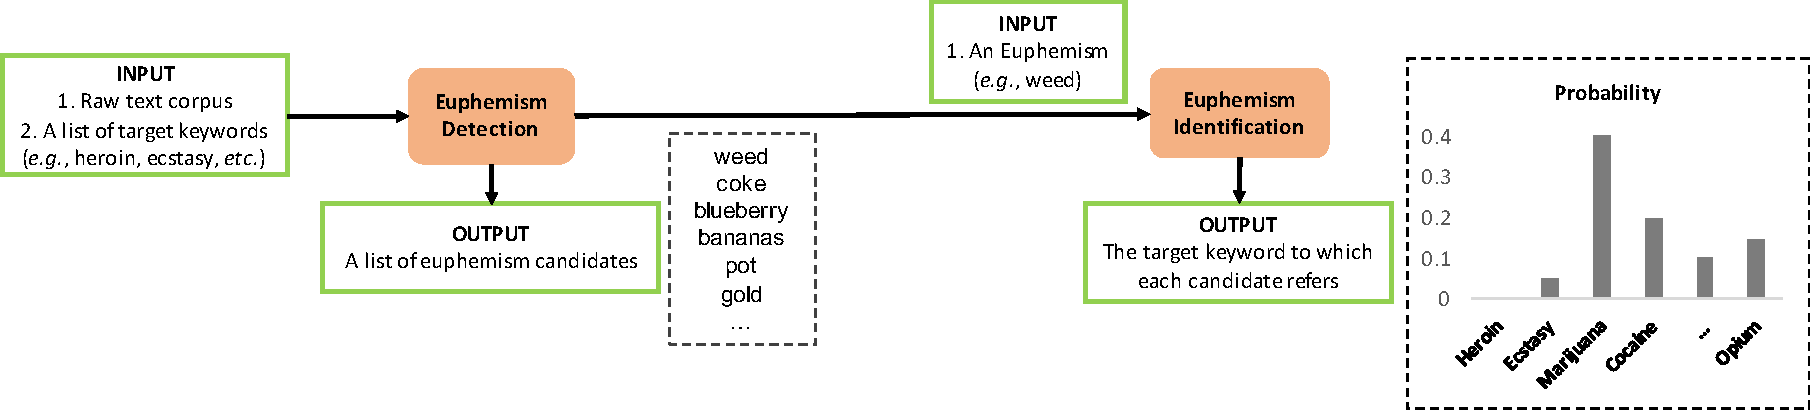
\includegraphics[width=1.00\linewidth]{figures/1}
	\caption{Euphemism detection and identification pipeline.}
	\label{fig:model_overview}
\end{figure*}

Our work is most closely related to four state-of-the-art approaches \cite{yuan2018reading,felt2020recognizing,taylor2017surfacing,magu2018determining}. 
CantReader \cite{yuan2018reading} aims to automatically identify ``dark jargon'' from cybercrime marketplaces. 
CantReader employs a neural-network based embedding technique to analyze the semantics of words, and detects euphemism candidates whose contexts in the background corpus (\eg, Wikipedia) are significantly different from those in the target corpus. 
Therefore, it takes as input a ``dark'' corpus (\eg, Silk Road anonymous online marketplace \cite{christin2013traveling} forum), a mixed corpus (\eg, Reddit), and a benign corpus (\eg, English Wikipedia). 
Different from CantReader, 
we assume only access to a single target corpus -- although we do rely on context-aware embeddings that could be pre-trained from a reference corpus like Wikipedia, and then fine-tuned to the target corpus.
More importantly, we find that our approach outperforms CantReader, presumably because we explicitly use context.
%does not achieve performance competitive with ours, presumably due to the fact that it does not make explicit use of context. 

Another relevant baseline \cite{felt2020recognizing} detects euphemisms instead by using sentiment analysis. 
It identifies a set of  euphemism candidates using a bootstrapping algorithm for semantic lexicon induction. 
Though the methodology seems reasonable and intuitive at first, it requires additional manual filtering process to refine the candidates and thus, fails to meet the requirement of automatic, large-scale detection 
that online content moderators desire. 
In yet another approach, Magu et al.\ \cite{magu2018determining} and Taylor et al.\ \cite{taylor2017surfacing} propose two algorithms that leverage word embeddings and community detection algorithms. 
Magu et al.\ \cite{magu2018determining} generates a cluster of euphemisms by the ranking metric of eigenvector centralities \cite{bonacich1972factoring,bonacich1972technique}.
Due to the intrinsic nature of the algorithm, this approach 
requires a starting euphemism seed to find others. 
Taylor et al.\ \cite{taylor2017surfacing} creates neural embedding models that capture the word similarities, uses graph expansion and the PageRank scores \cite{page1999pagerank} to bootstrap initial seed words, and finally enriches the bootstrapped words to learn out-of-dictionary terms that behave like euphemisms.
However, the approaches of Magu et al.\ \cite{magu2018determining} and Taylor et al.\ \cite{taylor2017surfacing} were tested on a single dataset.  
Unfortunately, 
we do not find their performance to be as strong on the multiple datasets we evaluate. 

%and we find their performance to be poor on all of  the datasets we evaluated.
% calling into question its effectiveness for other datasets and categories. 





\subsection{Euphemism Identification}
\label{sec:related_iden}
To the best of our knowledge, no work has explicitly attempted to infer euphemism meaning.
% except for a few peripheral works that identify the broad category of a euphemism. 
Yuan et al.\ \cite{yuan2018reading} tackles a related problem by identifying the hypernym of euphemisms (\eg, whether it refers to a drug or a person).
% It first extracts a set of hypernym candidates, and then run a classifier to determine the best candidate to serve as the hypernym of a euphemism. 
In a more general sense, the task of euphemism identification is also related to sense discovery of unknown words \cite{ishiwatari2019learning,ni2017learning} and word sense disambiguation \cite{taghipour2015semi,raganato2017neural,raganato2017word,iacobacci2016embeddings}. 
Sense discovery aims to understand the meaning of an unknown word by generating a definition sentence. 
Word sense disambiguation focuses on identifying which sense of a word is used in a sentence, given a set of candidate senses.
% and It is typically a form of multiple choice questions with distinct sense meanings. 
However, neither of these are able to capture nuanced differences between a group of semantically-similar target words in the same category. 

\subsection{Self-supervised Learning}
The technical innovations in our 
work rely heavily on  \emph{self-supervision}, a form of unsupervised learning where the data itself provides the supervision \cite{weng2019selfsup}. 
% We achieve euphemism identification by proposing a self-supervised learning algorithm, a form of unsupervised learning where the data itself provides the supervision \cite{weng2019selfsup}. 
% Below, we provide some background of self-supervised learning and review some important ideas and works. 
%\noindent \textbf{Self-supervised learning}: 
% Given a task and enough labels, supervised learning can typically solve it really well. 
% Supervised learning requires labelled data (\eg, ImageNet), which is expensive to obtain. %  and hard to be scaled up. 
Self-supervision was designed to make use of vast amounts of unlabelled data (\eg, free text, images) 
by constructing a supervised learning task from the data itself to predict some attribute of the data.
For example, to train a text prediction model, one can take a corpus of text, mask part of the sentence, and train the model to predict the masked part;
this workflow creates a supervised learning task from unlabelled data.
% An example might be to modify training samples in a controlled fashion and train a sub-model to identify the modification.
% The nature of the self-supervised task typically depends on the application. 
% For example, suppose we are training an image classifier and have only , we could train our model on modified 
% is substantially more than a limited number of human curated labelled datasets, it is wasteful not to use them. However, unsupervised learning is not easy and usually works much less efficiently than supervised learning.
%What if we can get labels for free for unlabelled data and train unsupervised dataset in a supervised manner? We can achieve this by framing a supervised learning task in a special form to predict only a subset of information using the rest. In this way, all the information needed, both inputs and labels, has been provided. This is known as self-supervised learning.
Self-supervision has been widely used in language modeling \cite{devlin2019bert,lan2019albert,liu2019roberta,baevski2020wav2vec,chen2020big,liu2018empower}, representation learning \cite{feng2019self,kolesnikov2019revisiting,sabokrou2019self}, robotics \cite{mees2019self,nair2017combining,berscheid2020self}, computer vision \cite{zhai2019s4l,sun2019unsupervised,xu2019self,yin2020dreaming} and reinforcement learning \cite{kahn2018self,zeng2018learning,pong2019skew}. 
One of our contributions is to generalize and extend the idea of self-supervision to the task of euphemism identification. 


% Self-supervised learning empowers us to exploit a variety of labels that come with the data for free. The motivation is quite straightforward. Producing a dataset with clean labels is expensive but unlabeled data is being generated all the time. To make use of this much larger amount of unlabeled data, one way is to set the learning objectives properly so as to get supervision from the data itself.



	%!TEX root = main.tex
% UTF-8 encoding
% \begin{figure*}[t]
% 	\centering
% 	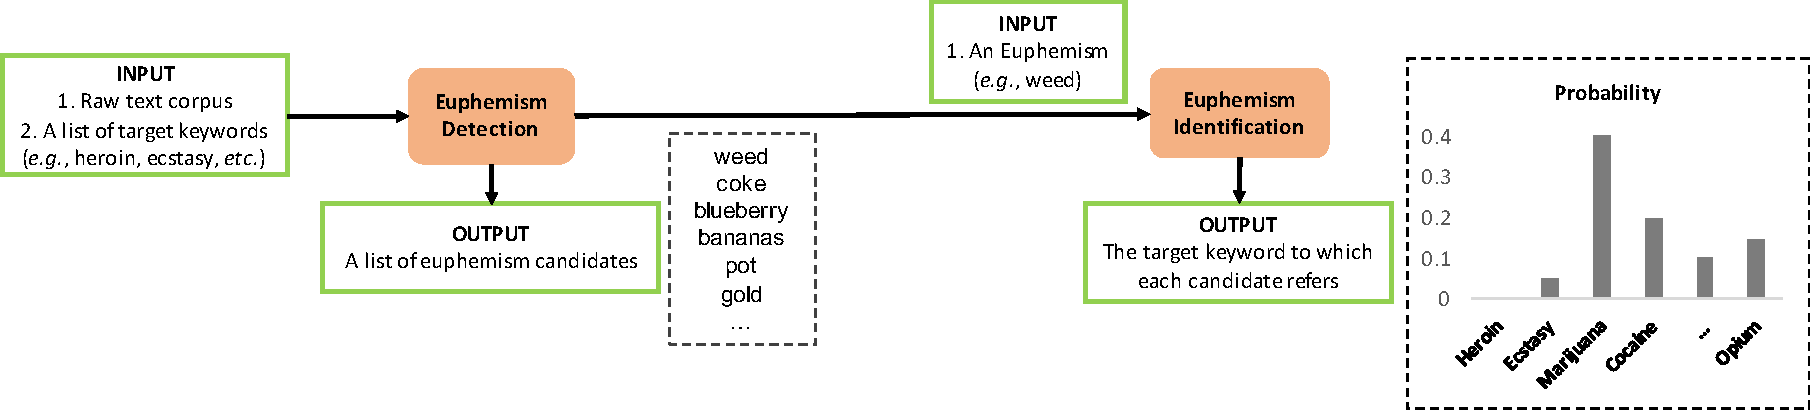
\includegraphics[width=0.98\linewidth]{figures/1}
% 	\caption{An overview of the task.}
% 	\label{fig:model_overview}
% \end{figure*}


\section{Problem Description}
\label{sec:problem}


In this study, we assume a content moderator that has access to a textual corpus (\eg, a set of posts from an online forum), 
and is required to moderate content related to a given list of target keywords. 
In practice, forum users may use \emph{euphemisms}---words that are used as substitutes for  one of the target keywords. 
We have two goals, euphemism detection and euphemism identification, defined as follows: 
1) \emph{Euphemism detection:} Learn which words are being used as euphemisms for keywords. A moderator can use this to filter content that may need to be moderated.
2) \emph{Euphemism identification:} Learn the meaning of euphemisms. This can be used by the moderator to understand context, and individually review content that uses euphemisms. 
% Our goal is to detect euphemisms in the corpus,   (\eg, a data dump from an online forum) and for each euphemism to identify the target keyword it refers to. 

As shown in Figure \ref{fig:model_overview}, these two tasks are complementary and form, together, a content moderation pipeline.
The euphemism detection task takes as input (a) the raw text corpus, and (b) a list of target keywords (\eg, heroin, marijuana, ecstasy, \etc). 
The expected output is an ordered ranked list of euphemism candidates, sorted by model confidence. 
% Once a euphemism is successfully detected, we are interested in identifying which target keyword it refers to, by a euphemism identification module. 
The euphemism identification module takes as input a euphemism (\eg, weed) and  outputs a probability distribution over the target keywords in the list. 
For example, if we feed the euphemism \emph{weed} into this module, the output should be a probability distribution over keywords, with most of the mass on \emph{marijuana}.
% Take ``weed'' as an example, we expect the identification module tells that it is more likely to be marijuana than other drugs. 


\noindent \textbf{Remark}: 
We use the term ``category'' to denote a 
topic (\ie, drug, weapon, sexuality). 
We use ``target keyword'' to refer to the specific keyword in each category users might be trying to use euphemisms for (\eg, ``marijuana'' and ``heroin'' are example of target keywords in the drug category). 

	%!TEX root = main.tex
% UTF-8 encoding

\section{Proposed Approach}
\label{sec:model}
We next discuss in detail our proposed euphemism detection approach in Section \ref{sec:model_det} and the proposed euphemism identification approach in Section \ref{sec:model_iden}. 


\subsection{Euphemism Detection}
\label{sec:model_det}
\begin{figure*}
	\centering
	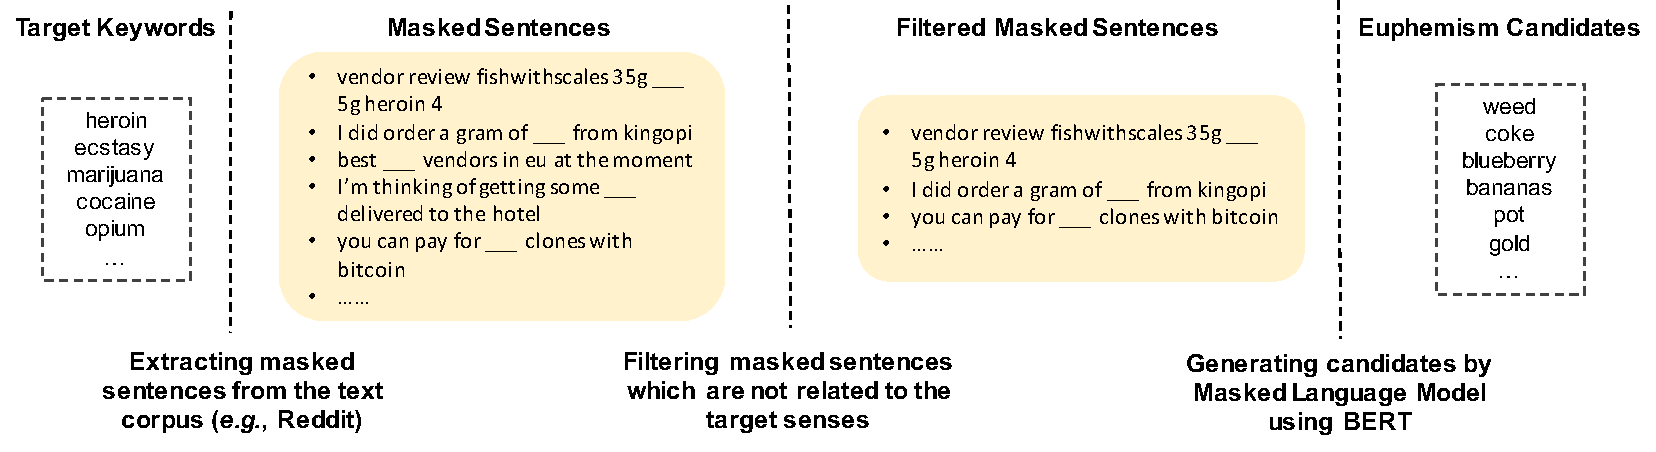
\includegraphics[width=1.0\linewidth]{figures/2}
	\caption{An overview of the euphemism detection framework.}
	\label{fig:model_det}
\end{figure*}

The challenge to euphemism detection is that euphemisms are typically innocent-looking, and their usage in a sentence is often natural and grammatical. %lies in the inability to identify them without having an explicit mapping between the words and their implied meanings. 
For instance, the words used as euphemisms with drug meanings tend to be words used in common parlance. 
%For example, ``blueberry'' could either mean a fruit, or marijuana depending on the context. Without the context, deciding whether a word is a euphemism or not would be impossible even for human experts. %For instance, \eg, 'one ounce of \textit{cheese}'). 
%\nicolasc{we said this already in the introduction, almost verbatim, do we need to repeat it here? by the same token, the proposed model (section III)  is useful but do we need to re-define euphemism detection and identification since we defined them in the introduction already?}
% Answer to Nicolas: changed it to a shorter version. 

Human experts (or even non-experts to a large extent) typically rely on information from the context to disambiguate the meaning of polysemous words. With this in mind,
much contemporary work on  euphemism detection has mainly relied on the implicit contextual information available in static word embeddings (\eg, word2vec) in combination with network analysis (\eg, community detection) \cite{taylor2017surfacing,magu2018determining}, using sentiment lexicons \cite{felt2020recognizing}, and relying on semantic comparison across corpora \cite{yuan2018reading}. 
However, the use of static word embeddings, which provides a single representation for a given word (without accounting for its polysemy), leads to an ineffective modeling of the acquired polysemy of the euphemisms. 

Going beyond the approaches in related prior work, we propose to detect euphemisms by explicitly harnessing their contextual information. Toward this, we formulate the problem as an unsupervised fill-in-the-mask problem and solve it using the idea of a Masked Language Model (MLM), an important modeling idea behind large pre-tained language models such as BERT \cite{devlin2019bert}. 

We carry out our proposed approach to euphemism detection in the following three stages (represented  in Figure~\ref{fig:model_det}): 
1) Extracting contextual information, 
2) Filtering out noisy masked sentences, and 
3) Generating euphemism candidates.  

\noindent\textbf{Contextual information extraction.} Taking as input all the target keywords, this stage first extracts the masked sentences of all the keywords. 
Here, a masked sentence refers to a sentence excluding the target keyword. 
Taking the first example sentence in Table~\ref{table:example3} as an example, the corresponding masked sentence is ``This 22 year old former [MASK] addict who i did drugs with was caught this night.''. 
A collection of all  masked sentences of the target keywords serves as the source of the relevant and crucial contextual information. 

\noindent\textbf{Denoising contextual information.} Not all masked sentences are equally informative. 
The extracted collection of the masked sentences is noisy because there may be  instances where the mask token (\ie, ``[MASK]'') can potentially be filled by more than one target term or words unrelated to the target terms. 
The fourth example sentence 
in Table~\ref{table:example3} is one such case, where the masked sentence ``Why is it so hard to find [MASK]?'' is not specific to a drug and the mask token can be filled  by many words, including nouns such as ``jobs'', ``gold'' and even pronouns such as ``him''. 
Such masked sentences (example sentences 4--6 
in Table~\ref{table:example3}) are generic and lack relevant  context for disambiguating a polysemous word. 
To filter such generic masked sentences, we leverage a Masked Language Model (MLM) proposed in BERT \cite{devlin2019bert}. 
An MLM aims to find suitable replacements of the masked token, and outputs a ranked list of potential replacement terms.  We fine-tune the `bert-base-uncased' pre-trained model\footnote{ \url{https://huggingface.co/transformers/model\_doc/bert.html\#bertformaskedlm}} to the language of the  of domain-specific body of text (for instance,  the collection of Reddit posts for the case of drug-related euphemisms).

Empirically, we find that if the masked sentence is specific to a target category (e.g., drug names), words related to the target category will be ranked highly in the replacement list. 
In contrast, if the masked sentence is generic, the highly ranked replacements are more likely  to be random words unrelated to the target category (\eg, ``jobs'', ``gold'', ``him''). 
Therefore, we set an MLM threshold $t$ to filter out the generic masked sentences. 
Considering the ranked list of replacements for the mask token, if any target keyword appears in the top $t$ replacement candidates for the masked sentence, we consider  the masked sentence to be a valid instance of a context. Otherwise, it is considered to be a generic one and filtered out. 
We set the threshold $t$ to be 5 in our experiments and discuss its  sensitivity in Section \ref{sec:dis_parameter_analysis}. 


\noindent\textbf{Candidate euphemism generation.} The informative masked sentences combined with a pre-trained language model that is fine-tuned to the text corpus of interest   provides the setting to  generate the euphemism candidates. 
%After fine-tuning the pretrained BERT language model on the collection of sentences with euphemism occurrences, we observe that the euphemisms are good replacements for the mask tokens. 
For each masked sentence denoted as $m$, and for each word candidate $c$ in the vocabulary (\ie, all words available in the BERT pre-trained model), we compute its MLM probability (the probability of the word occurring in $m$ as predicted by the language model) $h_{c,m}$  by a pre-trained BERT model.
Therefore, given a set of masked sentences, the weight $w_{c}$ of a word candidate $c$ is calculated as: 
$w_c = \sum_{m'}h_{c, m'}$. 
The final generation stage simply ranks all word candidates by their weights. 

To clarify, we use the masked language model twice---once for filtering the masked sentences and a second time for generating the euphemism candidates from the masked sentences. 


\subsection{Euphemism Identification}
\label{sec:model_iden}
\begin{figure*}
	\centering
	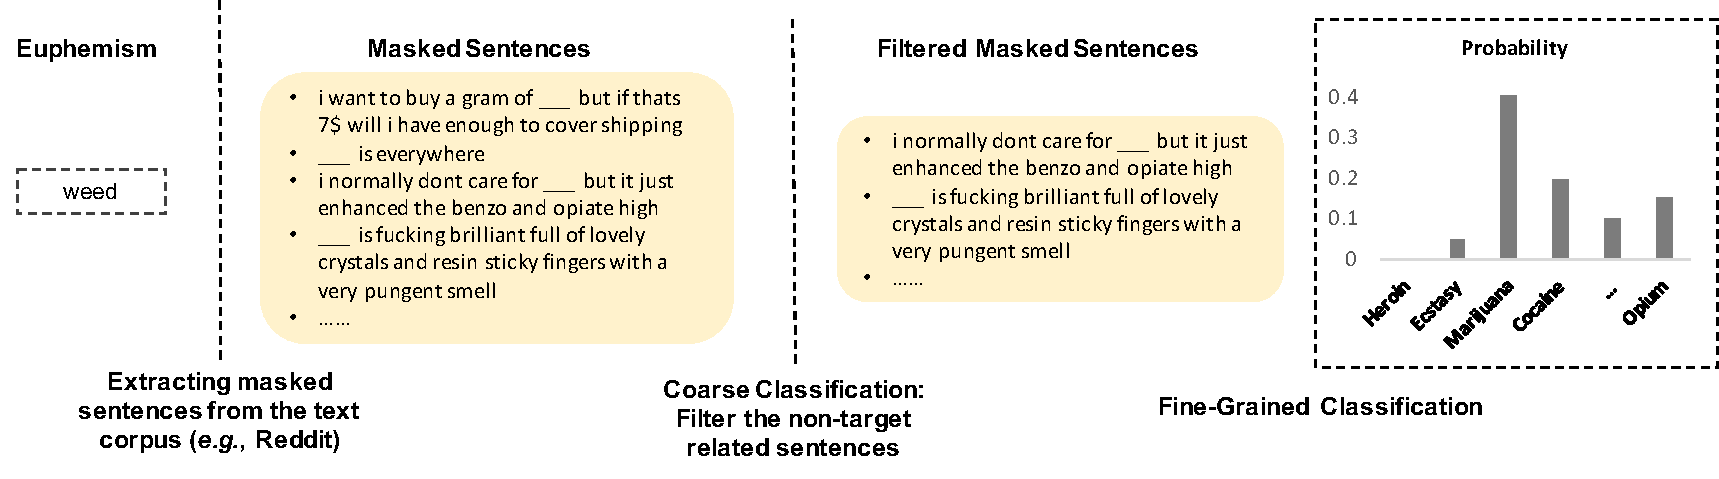
\includegraphics[width=1.00\linewidth]{figures/3}
	\caption{An overview of the euphemism identification framework.}
	\label{fig:model_iden}
\end{figure*}

Once the euphemisms are detected, we aim to identify what target keyword each euphemism refers to. 
Taking the second and third example sentences in Table \ref{table:example1}, we want to identify that ``coke'' refers to ``cocaine'' and  ``pot''  to  ``marijuana.'' 

We first discuss the challenges of the task (Section \ref{sec:iden_challenges}), and the  intuition of our approach to solve the problem (Section \ref{sec:intuition}). Finally, we present the training details of our approach (Section \ref{sec:iden_approach}). 

\subsubsection{Challenges}
\label{sec:iden_challenges}
%\noindent \textbf{Challenges}: 
Euphemism identification has been acknowledged as a highly challenging task \cite{yuan2018reading}, due to the following key challenges: 
\begin{itemize}%[leftmargin=*]
	\item \textit{Resource challenge}: 
	No curated datasets that are publicly available are adequate to exhaustively learn a growing list of mappings between euphemisms and their target keywords. Moreover, it is unclear what linguistic and ontological resources one would need to automate this task.  
	\item \textit{Linguistic challenge}: 
	The distinction in meaning between the target keywords  (\eg, cocaine and marijuana) is often subtle and difficult to learn from raw text corpora alone. 
	Even human experts are unable to accurately identify what a euphemism refers to by looking at a single  sentence. 
	On the other hand, having access to a larger number of  sentences where the euphemism occurs, provides more context to analyze the nuances between different contexts, and enables identifying what the euphemism refers to. 
	A second linguistic challenge is related to the ambiguity of the euphemism itself. 
	A given euphemism can  be used in a euphemistic or non-euphemistic sense, adding the extra layer of linguistic nuance (Table \ref{table:example4}). 
\end{itemize}


%To the best of our knowledge, no prior work has explicitly captured the meaning of a euphemism except for a few peripheral works   that identify the hypernym of a euphemism, as in ``sedative'' for a drug-related euphemism  (\eg, \cite{yuan2018reading}). 
%\nicolasc{didn't we say this in related work? paragraph candidate for deletion}
%Answer to Nicolas: removed. 

\subsubsection{Intuition}
\label{sec:intuition}
\WZ{Taking the awesome advices from Suma and Nicolas, I restructured the Intuition. How does it read now?}
We systematically address each of these challenges by a self-supervised learning scheme and a coarse-to-fine-grained classification framework. 
The key novelty lies in how we formulate the problem and solve it without additional linguistic resources or supervision. 

%To tackle the aforementioned challenges, a natural solution would be to avail a euphemism inventory---a list with each euphemism mapped to each target keyword---and then check whether the word is used euphemistically or not. % costly to collect the labels for every dataset. 
We address the \textit{resource challenge} with a self-supervised learning scheme. 
Self-supervised learning is a form of unsupervised learning where the data provides the supervision to automatically extract the training instances and their labels from an unlabeled raw text corpus. It permits scaling the large amount of 
More specifically, we extract all sentences that include the target keywords (\eg, cocaine, marijuana, heroin), mask the target keywords, and consider the masked sentences as training instances. 
This permits us to automatically construct a labeled dataset, where the instances are the masked sentences and their respective target keywords are labels. 

To address the \textit{linguistic challenge}, we adopt a coarse-to-fine-grained classification scheme, for its better discriminative performance in various tasks \cite{huo2019coarse,liu2018global,li2019exploiting}. 
The coarse classifier is a binary classifier, to examine whether the sentence is related to the specific category (\eg, drug) or not. 
It aims to filter out sentences where the euphemism words do not occur in a euphemistic sense. 
The fine-grained classifier is a multi-class classifier trained on the curated dataset from the self-supervised learning scheme, and aims to learn a specific mapping from the masked sentence to the target keyword. 



\noindent \textbf{Example}: 
Taking ``weed'' as an example, we aim to generate a probability distribution over target keywords, with most of the mass on marijuana (Figure \ref{fig:model_iden}). 
Assume that we already have a trained coarse classifier and a trained fine-grained classifer (training details will be discussed in Section \ref{sec:iden_approach}). 
We first extract all its masked sentences from the text corpus. 
Second, by the corase classifier, we filter those masked sentences that are not related to the target category (\ie, drug). 
Then, we use the filtered masked sentences as inputs to the fine-grained multi-class classifier, and obtain the target keyword label for each masked sentence. 
Now we have a list of labels for the euphemism ``weed'' (\eg, 36.1k times of marijuana, 4.2k times of ecstasy, \etc) and the final output is the label (target keyword) assigned to a majority of the euphemism's masked sentences, here \textit{marijuana}. % is a probability distribution over all the target keywords by the fraction of the number of labels. 


%To map the given euphemism to a specific target word, we construct a probability distribution over the target keywords, obtained as  the fraction of euphemism's masked sentences  labeled with a target keyword. 
%target keywords to which the masked sentences belong, is used to choose the target keyword that the euphemism maps to. 
%The target keyword with the highest probability is mapped to the euphemism.

%we adopt a supervised classification approach to learn, from their masked sentences, the nuances between different target keywords in the same category. 
%More specifically, we first train a multi-class classifier in a  self-supervised manner using the automatically labeled dataset, to learn a mapping from the masked sentence to the target keyword. 
%Then, for each euphemism, we extract its associated masked sentences, and obtain their target keyword labels using the trained classifier. 
%In the inference stage, different masked sentences for the same euphemism may be assigned different target keywords. 
%For each euphemism, we construct a probability distribution over the target keywords assigned by the classifier, where the probability of a euphemism being a target keyword is the fraction of masked sentences of that euphemism labeled with the target keyword. 
%%We consolidate the multiple labels corresponding to the masked sentences of a given euphemism by converting the hard decisions for the different instances into a soft decision over the target keywords. We do this by obtaining the   probability distribution over the target keywords, given by the fraction of times a given target keyword was chosen. 
%\nicolasc{I agree, I found this paragraph hard to understand; I didn't modify much, because I am not sure I understand well enough how the technique works.}
%\nicolasc{I got quite lost in the intuition. I wonder if it would make sense to use a running example based on one of the earlier tables to anchor the discussion.} 
%\SB{edited: how does it read now?}
%%Finally, the output will be a probability distribution by the percentage of the target keyword labels. 





\subsubsection{Training Details}
\label{sec:iden_approach}
Two classifiers need to be trained: 1) A coarse classifier to filter out the masked sentences of euphemism words not associated with their euphemistic sense
% (and hence use masked sentences related to the target keywords)
and, 2) A multi-class classifier to determine the target keyword to which the euphemism refers. 

\noindent \textbf{Coarse Classifier}: 
The coarse classifier is a binary classifier to determine whether a masked sentence is related to the target keywords or not. 
Obtaining the positive instances is easy; we collect all the masked sentences of the target keywords (\eg, we obtain the masked sentences from Table \ref{table:example3}). 
To obtain the negative instances, we adopt a negative sampling approach \cite{mikolov2013distributed}; 
we randomly choose a sentence in the text corpus and randomly mask a token. 
Since the corpus is large and diverse, we assume the randomly chosen masked sentence is not related to the target keyword. 
To create a balanced dataset, we select as many negative instances as there are positive ones. 
This set of positive and negative instances constitutes the training set, with masked sentences and their respective labels to indicate whether a masked sentence is related to the target keywords or not. 
We use 70\% of the data instances for training, 10\% for validation, and 20\% for testing. 
We select an LSTM recurrent neural network model \cite{hochreiter1997long} with an attention mechanism \cite{bahdanau2015neural} for its ability to learn where to pay attention in the input sequence. 
We obtain 98.8\% for the training accuracy and 90.1\% of the testing accuracy. 
Our experiments also included other classification models and we discuss our selection in Section \ref{sec:ablation_coarse}. 

\noindent \textbf{Multi-class Classifier}:
As presented above in Section~\ref{sec:intuition}, we use as inputs the masked sentences and as labels the target keywords. 
As an empirical selection, we adopt the multinomial logistic regression classifier \cite{hosmer2013applied} by representing each word as one-hot encoding and each sentence as the average of its composing words' encoding. 
By using the same data splitting ratio as the coarse classifier, we obtain about 55\% on training accuracy and 24\% on testing accuracy for the drug dataset (there are 33 target names in the drug dataset and therefore a random guess accuracy would be 3.3\%). 
Results by other classification models are discussed in Section \ref{sec:ablation_fine-grained}. 


	%!TEX root = main.tex
% UTF-8 encoding
\section{Empirical Evaluation}
\label{sec:res}
In this section, we empirically evaluate the performance of our proposed approach and compare with that a set of baseline models on both euphemism detection (in Section \ref{sec:res_det}) and euphemism identification (in Section \ref{sec:res_iden}). 

\subsection{Experimental Setup}
We implemented all  models in Python 3.7 and conducted all the experiments on a computer with twenty 2.9 GHz Intel Core i7 CPUs and one GeForce GTX 1080 Ti GPU. 
%Here we describe the datasets used in the study and the parameter settings of our system.

\noindent \textbf{Datasets}: 
We empirically validate our proposed model on  three separate datasets related to three broad areas of euphemism usage: drug, weapon, and sexuality. 
For the algorithm to be applicable to a dataset, we require two kinds of inputs: 1) the raw text corpus from which we extract the euphemisms and their masked sentences, and 2) a list of target keywords (\eg, heroin, marijuana, ecstasy, \etc). 
For the purpose of carrying out a quantitative evaluation of the euphemism detection and identification approaches and comparing them with prior art, we rely on a ground truth list of  euphemisms and their target keywords. Ideally, such a list  should contain all  euphemisms for the evaluation of euphemism detection, and a one-to-one mapping from each euphemism to its actual meaning, for the evaluation of euphemism identification. 

\begin{itemize}%[leftmargin=*]
	\item {\em Drug dataset}: We collected 1,271,907 posts from 46 distinct 
	``subreddits''\footnote{Forums hosted on the Reddit website, 
	and associated with a specific topic.} 
	related to drugs and dark web markets, 
	including the largest ones---``Bitcoin'' (565,614 posts), 
``Drugs'' (373,465 posts),
``DarkNetMarkets'' (125,300 posts),
``SilkRoad'' (22,989 posts), 
``DarkNetMarketsNoobs'' (22,699 posts). 
A number of these subreddits were banned from the platform 
in early 2018 \cite{cimpanu2018reddit}. 
Accordingly, the posts collected were authored between February 9, 2008 and December 31, 2017. 
While online drug trade dates back (at least) to USENET groups in the 1990s, 
it truly picked up mainstream traction with the emergence of the 
Silk Road in 2011. 
Our data corpus captures these early days, 
as well as the more mature ecosystem that followed 
\cite{soska15markets}.

	In addition, we obtained a list of drug names and the corresponding ground truth drug euphemism list from the Drug Enforcement Administration (DEA) \cite{drug2018slang}. 
	
	\item {\em Weapon dataset}: The raw text corpus comes from a combination of the 
	corpora collected by Zanettou et al.\ \cite{zannettou2018gab}, Durrett et al.\ \cite{durrett2017identifying} and the examples in Slangpedia\footnote{\url{https://slangpedia.org/}}. 
	The combined corpus has 310,898 posts. 
	Both the list of weapon target keywords and the respective euphemisms are obtained from The Online Slang Dictionary\footnote{\url{http://onlineslangdictionary.com/}}, Slangpedia, and The Urban Thesaurus\footnote{\url{https://urbanthesaurus.org/}}. 
	
	\item {\em Sexuality dataset}: The raw text corpus comes from the Gab social networking services\footnote{\url{https://gab.com/}}. We use 289,4869 processed posts, collected from Jan 2018 to Oct 2018.\footnote{Available at \url{https://files.pushshift.io/gab/}}
	%\nicolasc{did we collect this ourselves? if not who did?} 
	% Answer: it is available online. I am not sure who collects the data. 
	Both the list of sexuality target keywords and the euphemisms are obtained from The Online Slang Dictionary. 
\end{itemize}
%\nicolasc{An unknown commenter said ``Show some stats of the dataset?'' I agree and I did for Reddit, can we do the same for the others?}
%Answer: Thanks for pointing it out. Done. 


\subsection{Euphemism Detection}
\label{sec:res_det}
We evaluate the performance of euphemism detection in this section. 

\noindent \textbf{Evaluation Metric}: 
For each dataset, the input is an unordered list of target keywords and the output is an ordered ranked list of euphemism candidates. 
Given the nature of the output, we evaluate the output using the measure precision at $k$ ($P@k$), which is commonly used in information retrieval to evaluate how well the search results corresponded to a query \cite{manning2008introduction}. 
$P@k$, ranging from 0 to 1, measures the proportion of the top $k$ generated results that are correct (in our case, valid euphemisms). 
Because of the known shortcoming that $P@k$ fails to take into account the positions of the relevant documents \cite{jarvelin2017ir}, we report $P@k$ for multiple values of $k$ ($k=10, 20, 30, 40, 50, 60, 80, 100$) to resolve the issue. 

We point out that we are unable to measure recall for the following two reasons: 
1) Some euphemisms in the ground truth list do not appear in the text corpus at all and using recall as a measure can result in a misrepresentation of the performance of the approaches; 
2) Those euphemisms that indeed appear in the text corpus,  may not have been used in the euphemistic sense. 
For example, ``chicken" is a euphemism for ``methamphetamine", but it could have been used only in the animal sense in the corpus. 

%These two reasons also highlight why using a ground truth list for evaluation may not be the perfect way of evaluating the performance of proposed approaches. \SB{are we inviting trouble with this statement? If you think so, we can exclude it.} 
%These two reasons also underscore why  constructing a perfect ground truth list whereof all euphemism answers on the list have actually been used in the euphemistic sense in the text corpus it is extremely difficult to. 




\noindent \textbf{Baselines}: 
We compare our proposed approach with the following competitive baseline models:

\begin{itemize}%[leftmargin=*]
	%\setlength\itemsep{-0.2em}
	\item \textbf{Word2vec}: We use the word2vec algorithm \cite{mikolov2013distributed,mikolov2013efficient}  to learns the word embeddings for all the words  in the dataset. We then choose as euphemism candidates those words that are most similar to the input target keywords, in terms of  cosine similarity. 
	\item \textbf{TF-IDF + word2vec}: Instead of treating all the words in the dataset equally, this method first ranks the words by their potential to be euphemisms. Toward this, we calculate the TF-IDF weights of the words \cite{manning2008introduction} with respect to a background corpus (\ie, Wikipedia\footnote{\url{https://dumps.wikimedia.org/enwiki/}}), which captures a combination of the frequency of a word and its distinct usage in a given corpus. The idea is inspired by the assumption that words ranked higher in the target corpus (based on an appropriate metric, e.g., frequency) have a greater chance of being euphemisms than those ranked lower \cite{magu2018determining}.  We then select the euphemism candidates by following the word2vec approach above.  
	\item \textbf{CantReader}\footnote{\url{https://sites.google.com/view/cantreader}} \cite{yuan2018reading} employs a neural-network based embedding technique to analyze the semantics of words, detecting the euphemism candidates whose contexts in the background corpus (\eg, Wikipedia) are significantly different from those in the dark corpus. 
	\item SentEuph \cite{felt2020recognizing} recognizes euphemisms by the use of sentiment analysis. It lists a set of euphemism candidates using a bootstrapping algorithm for semantic lexicon induction. For a fair comparison with our approach, we do not include the manual filtering stage of the algorithm proposed by Felt and Riloff \cite{felt2020recognizing}. 
	\item \textbf{EigenEuph} \cite{magu2018determining} leverages word embeddings and a community detection algorithm, to generate a cluster of euphemisms by the ranking metric of eigenvector centralities. %\cite{bonacich1972factoring,bonacich1972technique}. 
	\item \textbf{GraphEuph}\footnote{\url{https://github.com/JherezTaylor/hatespeech_codewords}} \cite{taylor2017surfacing} also identifies euphemisms using word embeddings and a community detection algorithm. Specifically, it creates neural embedding models that capture word similarities, uses graph expansion and the PageRank scores \cite{page1999pagerank} to bootstrap an initial set of seed words, and finally enriches the bootstrapped words to learn out-of-dictionary terms that behave like euphemisms. 
	\item \textbf{MLM-no-filtering} is an adaptation of our approach and has the same architecture as our proposed approach. However, instead of filtering the noisy masked sentences, it uses all available masked sentences to generate euphemism candidates. 
\end{itemize}

For a fair comparison, we experimented with different combinations of parameters and report the best performance for each baseline method. 

\noindent \textbf{Results}: 
Table \ref{table:res_dec} summarizes the euphemism detection results. 
Our proposed approach outperforms all other baselines significantly in all evaluation measures and all three datasets. 

Among the baselines, the most robust ones are TF-IDF + word2vec, EigenEuph \cite{magu2018determining} and MLM-no-filtering. 
Compared with Word2vec, the TF-IDF + word2vec algorithm identifies a set of potential euphemisms first by calculating the TF-IDF with a background corpus (\ie, Wikipedia). 
The pre-selection step works well on the Drug and Sexuality datasets. 
Yet, it does not contribute much for the Weapon dataset. 
We think one of the possible reasons is that the euphemisms do not occur very frequently in the text corpus and therefore, do not rank high by TF-IDF scores. 


SentEuph \cite{felt2020recognizing} has poor performance in that it requires additional manual filtering stage to refine the results. 
GraphEuph \cite{taylor2017surfacing} has highly unstable results across datasets. 
Taylor \etal \cite{taylor2017surfacing} show that GraphEuph is tested on one dataset only (\ie, hate speech dataset on Twitter), calling in question its effectiveness on generalization to other domains. 
CantReader \cite{yuan2018reading} requires additional corpus to make the semantic comparison. 
However, we note that the results of CantReader are brittle to parameter tuning. 
We are unable to reproduce any results as competitive as reported by Yuan \etal \cite{yuan2018reading}, even through private communications with the authors. 
By comparing the performance of our approach and the ablation MLM-no-filtering, we conclude that the filtering step is effective in eliminating the noisy masked sentences and is necessary for producing quality and reliable results. 



\begin{table*}[ht!]
	\centering
	\small
	\caption{Results on euphemism detection. Best results are in bold.}
	\begin{tabular}{c|c|cccccccc}
		\toprule
		%\multicolumn{2}{c}{}& \multicolumn{5}{c}{\textbf{Effectiveness}} & \multicolumn{6}{|c}{\textbf{Diversity}} & \multicolumn{1}{|c}{\textbf{Rel.}} & \multicolumn{1}{|c}{\textbf{LQ.}}\\ 
		\multicolumn{2}{c}{}& \textbf{$P@10$}  & \textbf{$P@20$} &  \textbf{$P@30$} &  \textbf{$P@40$} & \textbf{$P@50$}  & \textbf{$P@60$} &  \textbf{$P@80$} &  \textbf{$P@100$}\\
		\midrule
		%\cmidrule{2-10} 
		
		\multirow{8}{*}{\rotatebox[origin=c]{90}{\textbf{Drug}}}
		&\textbf{Word2vec} & 0.10 & 0.10 & 0.09 & 0.09 & 0.08 & 0.09 & 0.08 & 0.09 \\
		&\textbf{TF-IDF + word2vec} & 0.30 & 0.25 & 0.20 & 0.20 & 0.16 & 0.17 & 0.16 & 0.18 \\
		&\textbf{CantReader \cite{yuan2018reading}} & 0.00 & 0.00 & 0.07 & 0.10 & 0.08 & 0.12 & 0.12 & 0.10 \\
		&\textbf{SentEuph \cite{felt2020recognizing}} & 0.10 & 0.10 & 0.07 & 0.05 & 0.08 & 0.07 & 0.09 & 0.07 \\
		&\textbf{EigenEuph \cite{magu2018determining}} & 0.30 & 0.30 & 0.30 & 0.25 & 0.22 & 0.22 & 0.20 & 0.19 \\
		&\textbf{GraphEuph \cite{taylor2017surfacing}} & 0.20 & 0.15 & 0.13 & 0.13 & 0.14 & 0.17 & 0.14 & 0.11 \\
		&\textbf{MLM-no-filtering} & 0.30 & 0.30 & 0.28 & 0.30 & 0.26 & 0.26 & 0.28 & 0.26 \\
		&\textbf{Our Approach} & \textbf{0.50} & \textbf{0.45} & \textbf{0.47} & \textbf{0.42} & \textbf{0.46} & \textbf{0.42} & \textbf{0.38} & \textbf{0.36} \\
		\midrule
		
		\multirow{8}{*}{\rotatebox[origin=c]{90}{\textbf{Weapon}}}
		&\textbf{Word2vec} & 0.30 & 0.30 & 0.27 & 0.23 & 0.18 & 0.20 & 0.20 &  0.18\\
		&\textbf{TF-IDF + word2vec} & 0.30 & 0.25 & 0.20 & 0.17 &  0.16 & 0.18 & 0.20 & 0.18 \\
		&\textbf{CantReader \cite{yuan2018reading}} & 0.20 & 0.20 & 0.17 & 0.18 & 0.16 & 0.17&0.13 & 0.11\\
		&\textbf{SentEuph \cite{felt2020recognizing}} & 0.00 & 0.00 & 0.03 & 0.05 & 0.06 & 0.05 & 0.05 & 0.04\\
		&\textbf{EigenEuph \cite{magu2018determining}} & 0.30 & 0.20  & 0.13 & 0.10 & 0.08 & 0.07 & 0.05 & 0.04\\
		&\textbf{GraphEuph \cite{taylor2017surfacing}} &  0.00 & 0.05 & 0.03 & 0.05 & 0.04 & 0.03 & 0.03 & 0.02\\
		&\textbf{MLM-no-filtering} & 0.30 & 0.30 & 0.20 & 0.17 & 0.18 & 0.18 & 0.15 & 0.15 \\
		&\textbf{Our Approach} & \textbf{0.40} & \textbf{0.45} & \textbf{0.37} & \textbf{0.35} & \textbf{0.32} & \textbf{0.28} & \textbf{0.25} & \textbf{0.20} \\
		\midrule
		
		\multirow{8}{*}{\rotatebox[origin=c]{90}{\textbf{Sexuality}}}
		&\textbf{Word2vec} & 0.10 & 0.05 & 0.07 & 0.08 & 0.08 & 0.08 & 0.09 &  0.09 \\
		&\textbf{TF-IDF + word2vec} & 0.40 & 0.25 & 0.20 & 0.20 & 0.20 & 0.17 & 0.15 & 0.13  \\
		&\textbf{CantReader \cite{yuan2018reading}} & 0.10 & 0.10 & 0.07 & 0.08 & 0.06 & 0.08 & 0.09 & 0.10 \\
		&\textbf{SentEuph \cite{felt2020recognizing}} & 0.10 & 0.10 & 0.08 & 0.10 & 0.08 & 0.10 & 0.08 & 0.06\\
		&\textbf{EigenEuph \cite{magu2018determining}} & 0.20 & 0.15 & 0.13 & 0.15 & 0.16 & 0.18 & 0.14 & 0.11\\
		&\textbf{GraphEuph \cite{taylor2017surfacing}} & 0.00 & 0.00 & 0.03 & 0.05 & 0.04 & 0.03 & 0.04 & 0.03 \\
		&\textbf{MLM-no-filtering} & 0.50 & \textbf{0.40} & 0.30 & 0.23 & 0.22 & 0.22 & 0.19 & 0.15 \\
		&\textbf{Our Approach} & \textbf{0.70} & \textbf{0.40}& \textbf{0.33}& \textbf{0.33}& \textbf{0.28}& \textbf{0.25}& \textbf{0.23}& \textbf{0.19} \\
		\bottomrule
	\end{tabular}
	\label{table:res_dec}
\end{table*}



\subsection{Euphemism Identification}
\label{sec:res_iden}
For each euphemism that we have successfully detected, we now evaluate the results of euphemism identification. 

\noindent \textbf{Evaluation Metric}: 
For each euphemism, we generate a probability distribution over all target keywords and therefore, obtain a ranked list of the target keywords. 
We evaluate the Top k accuracy ($Acc@k$), which measures how often the ground truth class falls in the top k values of our generated ranked list. 


\noindent \textbf{Baselines}: 
Since there is a lack of related works in the research area of euphemism identification, we establish a few baseline methods and compare our proposed approach with them. 

\begin{itemize}%[leftmargin=*]
	\item Word2vec: for each euphemism, we select its closest target keyword in terms of the cosine similarities of the word embeddings. We use the word2vec algorithm \cite{mikolov2013distributed,mikolov2013efficient} to train on the text corpus to obtain word embeddings. 
	\item Clustering + word2vec: for each euphemism, we cluster all its masked sentences by k-means (we set $k=2$) algorithms. We aim to filter out the noisy masked sentences that are not related to the target keywords. Then, we compare the word2vec cosine similarities between the embeddings of the masked sentences of the euphemism and the target keywords. The most similar target keyword is selected for identification. 
	\item Binary + word2vec: similar to our approach, we use a binary classifier to filter out noisy masked sentences that are not related to the target keywords. Then, we use word2vec to find its closest target keyword. 
	\item Multi-class-only is an adaption of our approach. It has only the fine-grained multi-class classifier but no coarse classifier. 
\end{itemize}


\noindent \textbf{Results}: 
Table \ref{table:res_iden} summarizes the euphemism identification results. 
There are 33, 9, 12 categories for the drug, weapon and sexuality datasets respectively, resulting in the random guess performance for $Acc@1$ to be 0.03, 0.11, 0.08. 
Our algorithm achieves the best performance for all three datasets and has a large margin over the random guess performance. 


Word2vec has a bad performance, in that it is unable to capture the nuance differences between the target keywords by taking all sentences into consideration. 
Therefore, we construct two baselines (\ie, Clustering + word2vec and Binary + word2vec) to remove the noisy sentences and make the learning easier. 
Empirically, we find that the clustering algorithm does not work well whereas a binary classifier contributes to the performance improvement much. 
By inspecting the performance of clustering, we observe one issue that could cause the ineffectiveness of removing the noisy sentences. 
The k-means clustering algorithm did not cluster the sentences into a target keyword cluster and a non-target keyword cluster. Take the drug dataset as an example, we expect the two resulting clusters to be one drug-related cluster and one non-drug-related cluster. However, due to the broad context and vocabularies in the dataset, we find the clustering does not perform in such a way. The clustering might have been done in quality good \textit{vs.} non-quality good, or good feeling \textit{vs.} bad feeling and so on. Therefore, the k-means clustering fails to serve as a way to filter the non-drug-related masked sentences and leads to no performance improvement. 
In contrast, the binary classifier, which can be taken as a directed k-mean clustering algorithm, specifically filters out the non-drug-related sentences and therefore, shows strong improvement. 
In such a task, one can think that the performance of using a binary classifier is the upper bound of the performance by using a clustering algorithm. 


We would like to highlight two important findings: 
1) Comparing the results of Word2vec and Multi-class-only, we demonstrate the power of using a classification alrgorithm over an unsupervised word embedding learning method; 
2) by comparing the differences between Word2vec and Binary + word2vec and the differences between Multi-class-only and our approach, we demonstrate the discriminative power of a binary filtering classifier and therefore, show the benefit of using a coarse-to-fine-tuned classification over the vanilla multi-class classification. 



\begin{table}[ht!]
	\centering
	\small
	\caption{Results on euphemism identification. Best results are in bold.}
	\begin{tabular}{c|c|ccc}
		\toprule
		\multicolumn{2}{c}{}& \textbf{$Acc@1$}  & \textbf{$Acc@2$} &  \textbf{$Acc@3$} \\
		\midrule
		
		\multirow{5}{*}{\rotatebox[origin=c]{90}{\textbf{Drug}}}
		&\textbf{Word2vec} & 0.07 & 0.14 & 0.21 \\
		&\textbf{Clustering + word2vec} & 0.06 & 0.15 & 0.25 \\
		&\textbf{Binary + word2vec} & 0.13 & 0.22 & 0.30 \\
		&\textbf{Multi-class-only} & 0.11 & 0.19 & 0.26 \\
		&\textbf{Our approach} & \textbf{0.20} & \textbf{0.31} & \textbf{0.38} \\
		\midrule		
		
		\multirow{5}{*}{\rotatebox[origin=c]{90}{\textbf{Weapon}}}
		&\textbf{Word2vec} & 0.10 & 0.27 &  0.40 \\
		&\textbf{Clustering + word2vec} & 0.11 & 0.25 & 0.37 \\
		&\textbf{Binary + word2vec} & 0.22 & 0.43 & 0.57 \\
		&\textbf{Multi-class-only} & 0.25  & 0.40 & 0.61 \\
		&\textbf{Our approach} & \textbf{0.33} & \textbf{0.51} & \textbf{0.67} \\
		\midrule
		
		\multirow{5}{*}{\rotatebox[origin=c]{90}{\textbf{Sexuality}}}
		&\textbf{Word2vec} & 0.17 & 0.22 & 0.42 \\
		&\textbf{Clustering + word2vec} & 0.15 & 0.30 & 0.49 \\
		&\textbf{Binary + word2vec} & 0.21 & 0.39 & 0.59 \\
		&\textbf{Multi-class-only} &  0.19 & 0.40 & 0.51 \\
		&\textbf{Our approach} & \textbf{0.32} & \textbf{0.55} & \textbf{0.64} \\
		\bottomrule
	\end{tabular}
	\label{table:res_iden}
\end{table}




	%!TEX root = main.tex
% UTF-8 encoding
\section{Discussion}
\label{sec:dis}
Our algorithms rely on a small number of hyper-parameters and choices of classification models. 
In this  section, we demonstrate how to choose these hyper-parameters through detailed ablation studies, primarily on  the drug dataset.
% The discussion primarily relies on the drug dataset, owing to the fact 
% that drug-related euphemisms are numerous and evolve very rapidly. 

\subsection{Ablation Studies for Euphemism Identification}
As discussed above, we adopt a coarse-to-fine-grained classification scheme for euphemism identification, relying on two classifiers used in cascade. 
We discuss here the performance of multiple classifiers on both coarse and fine-grained classification. 

\subsubsection{Coarse Classifiers}
\label{sec:ablation_coarse}
\begin{figure}[ht!]
	\centering
	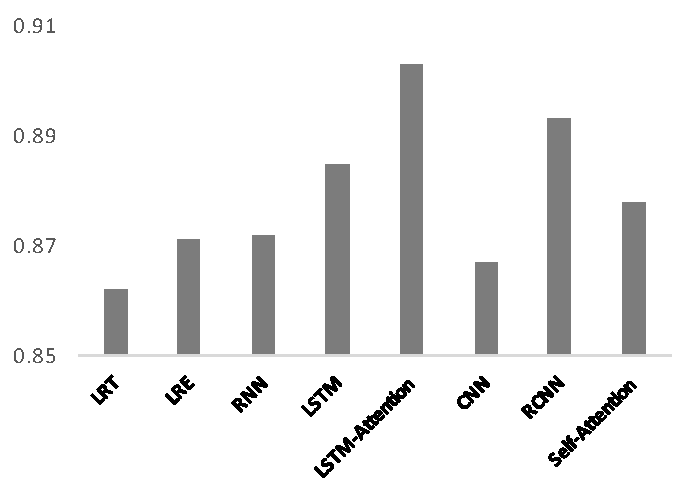
\includegraphics[width=0.7\linewidth]{figures/11}
	\caption{Testing accuracy for the coarse classifier.}
	\label{fig:11}
\end{figure}

In the euphemism identification framework, we use a binary classifier to filter out the sentences where euphemisms are used in non-euphemistic senses. 
We experiment with the binary classifiers shown below. Note that for all the neural models, we use 100-dimensional GloVe embeddings \cite{pennington2014glove} pre-trained on Wikipedia\footnote{\url{https://nlp.stanford.edu/projects/glove/}} and tune the embeddings by the models. 
\begin{itemize}
	\item Logistic Regression \cite{hosmer2013applied} on raw text (LRT): we first represent each word as a one-hot vector and then represente each sentence as the average of its member words' encodings. 
	\item Logistic Regression on text embeddings (LTE): we learn the word embeddings (100-dimensional) using word2vec \cite{mikolov2013distributed,mikolov2013efficient}. 
	We represent each sentence by the average of its member words' embeddings. 
	\item Recurrent Neural Network (RNN) \cite{rumelhart1985learning}: we use a 1-layer bidirectional RNN with 256 hidden nodes. 
	\item Long Short-Term Memory (LSTM) \cite{hochreiter1997long}: we use a 1-layer bidirectional LSTM with 256 hidden nodes. 
	\item LSTM-Attention: we add an attention mechanism \cite{bahdanau2015neural} on LSTM. 
	%The attention model computs soft alignment scores between each of the hidden_state and the last hidden_state of the LSTM.
	\item Convolutional Neural Networks (CNN) \cite{kim2014convolutional}: we train a simple CNN with one layer of convolution on top of word embeddings. 
	\item Recurrent Convolutional Neural Networks (RCNN) \cite{lai2015recurrent}: we apply a bidirectional LSTM and employ a max-pooling layer across all sequences of texts. 
	\item Self-Attention \cite{lin2017structured}: Instead of using a vector, we use a 2-D matrix to represent the embedding, with each row of the matrix attending on a different part of the sentence. 
\end{itemize}


We split the datasets into 70-10-20 for training, validation and testing. 
The model parameters are tuned on the validation data. 
Empirically, we find the LSTM-Attention performs the best across three datasets. This is  why we ultimately selected it and reported results using it in Section~\ref{sec:res}. 
Yet, as shown in Figure \ref{fig:11}, other classifiers have satisfactory performance as well, and reach a testing accuracy ranging from 0.86 to 0.90. 

\subsubsection{Fine-Grained Classifiers}
\label{sec:ablation_fine-grained}
In the euphemism identification framework, we use a multi-class classifier to identify to which target keyword each euphemism refers. 
Again, we experimented with the same set of classifiers as above.
Interestingly, we find that, for fine-grained classification, 
all classifiers have highly similar results. 
One possible reason is that each class has relatively small number of training instances (ranging from a few hundreds to 100k), which limits the discriminative power of advanced algorithms. 
For the drug dataset (33 target keywords), the training accuracy is about 55\% and the testing accuracy is about 24\%. 
This shows the feasibility of the task since the random guess accuracy would be 3.3\%. 
Given the similar performance across  classifiers, we recommend  Logistic Regression on raw text for better computational efficiency. 



\subsection{Parameter Analysis}
\label{sec:dis_parameter_analysis}
\begin{figure}[ht!]
	\centering
	\vspace{-0.5cm}
	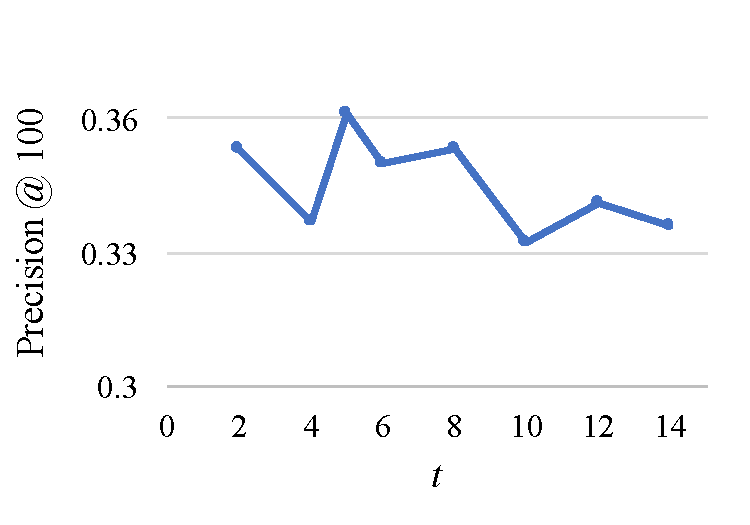
\includegraphics[width=0.7\linewidth]{figures/12}
	\caption{Sensitivity of $t$.}
	\label{fig:12}
\end{figure}

In the euphemism detection step 
(Section \ref{sec:model_det}), 
we set a masked language model threshold~$t$ to filter out the generic masked sentences. 
In the ranked list of replacements for the mask token, if any target keyword appears in the top-$t$ 
replacement candidates for the masked sentence, 
we consider  the masked sentence a valid context instance. % for the context of interest. 
Otherwise, we considere  the masked sentence generic and filter it out. 
Figure \ref{fig:12} shows how the results change with the threshold $t$ and we observe a slight decrease when the threshold $t$ is larger than 5. So, $t=5$ appears to be an optimal parameter choice.


\subsection{Limitations} 
While our approach for euphemism detection and identification
appears highly promising,
it does have some limitations.

\medskip 
\noindent{\textbf{Text-only moderation}}: 
Our approach only works with text, and our techniques
are not easily generalizable to other media.
Social media posts frequently include images, video, and audio,
which can be even more challenging (and even more traumatic)
to moderate by hand~\cite{newton2019terror, newton2019trauma, ofcom:ai2019}.
However, text is frequently associated with these other media, 
\eg, in the form of comments, and thus detecting euphemism use might 
indirectly provide clues to content moderators dealing with 
different media. 

\medskip
\noindent{\textbf{Other contexts}}:
Our approach performs well
on corpora discussing drugs, weapons, and sexuality.
In preliminary experiments
with a corpus of hate speech
it did not perform nearly as well,
producing many false matches
when tasked with identifying racial slurs.
We believe this is because
euphemisms related to drugs, weapons, and sex
typically have specific meanings;
\eg, ``pot'' always refers to marijuana, not some other drug.
Racial slurs, on the other hand,
are (in this corpus)
used imprecisely, and interchangeably with generic swearwords,
which seems to confuse euphemism identification.
We do not know yet whether this is a fundamental limitation.
Even if it is, though,
there are many  contexts where euphemisms have specific meanings
and our approach should be effective,  particularly forums selling illicit goods.
% :
% we are, for instance, planning to test it
% on a corpus of posts from ``darknet'' forums
% discussing credit card fraud and similar crimes.

\medskip
\noindent{\textbf{Robustness to adversarial evasion}}: 
In our evaluation, we have relied on \textit{a priori} 
non-adversarial datasets, 
that were gleaned from public, online forums. 
In other words, people were using euphemisms, 
but we do not know whether they were using them
specifically to evade content moderation.
Perhaps these euphemisms are, for them,
simply the ordinary names of certain things
within the circle where they were discussing them.
(Someone who consistently spoke of ``marijuana'' instead of ``pot''
on a forum dedicated to discussing drug experiences
might well be suspected of being an undercover cop.)

Because our algorithms rely on sentence-level context
to detect and identify euphemisms,
an adversary would need to change that context
to escape detection.
Such changes 
may also render the text unintelligible
to its intended audience.
Therefore, we expect our techniques
to be moderately resilient to adversarial evasion.
However, we cannot test our expectations at the moment,
since we do not have a dataset
where people were purposely using euphemisms
\emph{only} to escape detection.

\medskip
\noindent{\textbf{Usability for content moderators}}:
While our approach shows encouraging performance in lab tests,
we have not yet evaluated
whether it is good enough to be helpful to content moderators in practice.
That evaluation would require a user study of professional content moderators.
This is out of scope for the present paper,
which  focuses on the technical underpinnings
of euphemism detection and identification.
We are interested in investigating usability as a follow-up study.

% Detection Challenges
% Identification Challenges




%\subsection{Limitation and Future Work}
%%We run our experiments on two other datasets with relatively negative results. 
%Euphemistic phrase detection. 




%\subsection{The Effect of Fine-tuning the BERT Model}
%\begin{figure}[ht!]
%	\centering
%	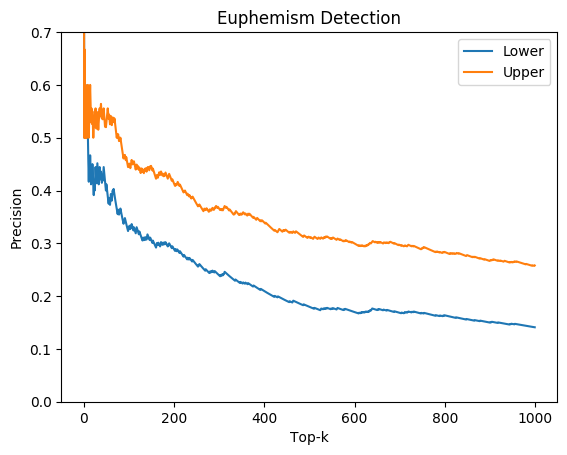
\includegraphics[width=0.48\linewidth]{figures/Precision_reddit}
%	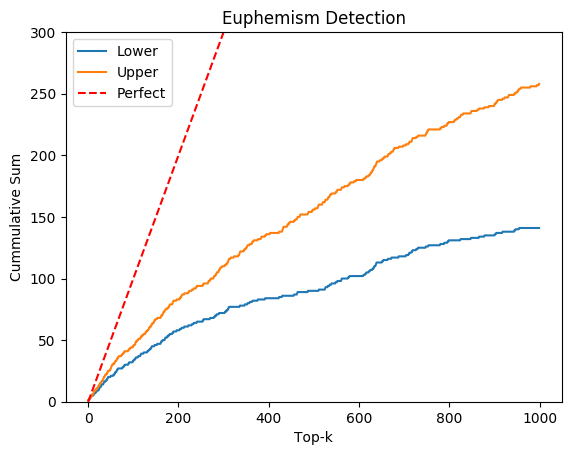
\includegraphics[width=0.48\linewidth]{figures/CSum_reddit}
%	\caption{Left shows the top-k precision \textit{vs.} k on the drug dataset. Right shows the cumulative correct numbers \textit{vs.} k on the drug dataset. }
%	\label{fig:precisionreddit}
%\end{figure}
%We have shown the numeric results of euphemism detection in Table \ref{table:res_dec}. Besides, we show the plots on top-k precision and cummulative correct detections against k in Figure \ref{fig:precisionreddit}. 



%\subsection{Computational Efficiency}
%We did not measure the baselines so far. 
%We implemented all models in Python 3.7 and conducted all the experiments on a computer with twenty 2.9 GHz Intel Core i7 CPUs and one GeForce GTX 1080 Ti GPU. 
%The BERT fine-tuning on the text corpus step took 5.4 hours (3 epochs).
%The euphemism detection took 1.5 hours. 
%The euphemism identification took 1.5 hours. 


	%!TEX root = main.tex
% UTF-8 encoding

\section{Conclusion}
\label{sec:conclusion}
Good paper. 



\section*{Reproducibility}
The code and pre-trained models are available at an anonymous link: \url{Some Anonymous Github Link}. 
We will make them publicly available upon the acceptance of the paper. 
	
	
	% IEEE specifies use of \section* for acknowledgments.
	\section*{Acknowledgments}
	\ifanonymized
	Omitted for anonymous submission.
	\else
	Acknowledgments go here.
	\fi
	
	% In rough-draft mode, start the bibliography on a new page, to make it
	% more obvious how close we are to the page limit.
	% Oakland 2020 page limit is 13 pages of main text + 5 pages of
	% bibliography and appendices.
	\ifroughdraft\clearpage\fi
	\clearpage
	
	% activate tweaks from main.bib
	\bstctlcite{ieeetran:tweaks}
	
	% References should always be sorted alphabetically, I don't care
	% if IEEE's official style guide says otherwise.
	\bibliographystyle{IEEEtranS}
	\bibliography{main}
	%%!TEX root = main.tex
% UTF-8 encoding

\newpage
\appendix

\begin{table*}
	\centering
	\caption{Euphemism detection results by our approach (better viewed in color). 
		Purple bold words are correctly detected euphemisms and on the ground truth list (\ie, the DEA list). 
		The purple underlined words indicate that they are incorrect by themselves, but are contained in true euphemism phrases, such as ``dog food", ``Chinese Tobacco" (euphemisms for ``heroin" and ``opium" respectively). 
		Those words which do not appear in the ground truth list are marked black. 
		}
	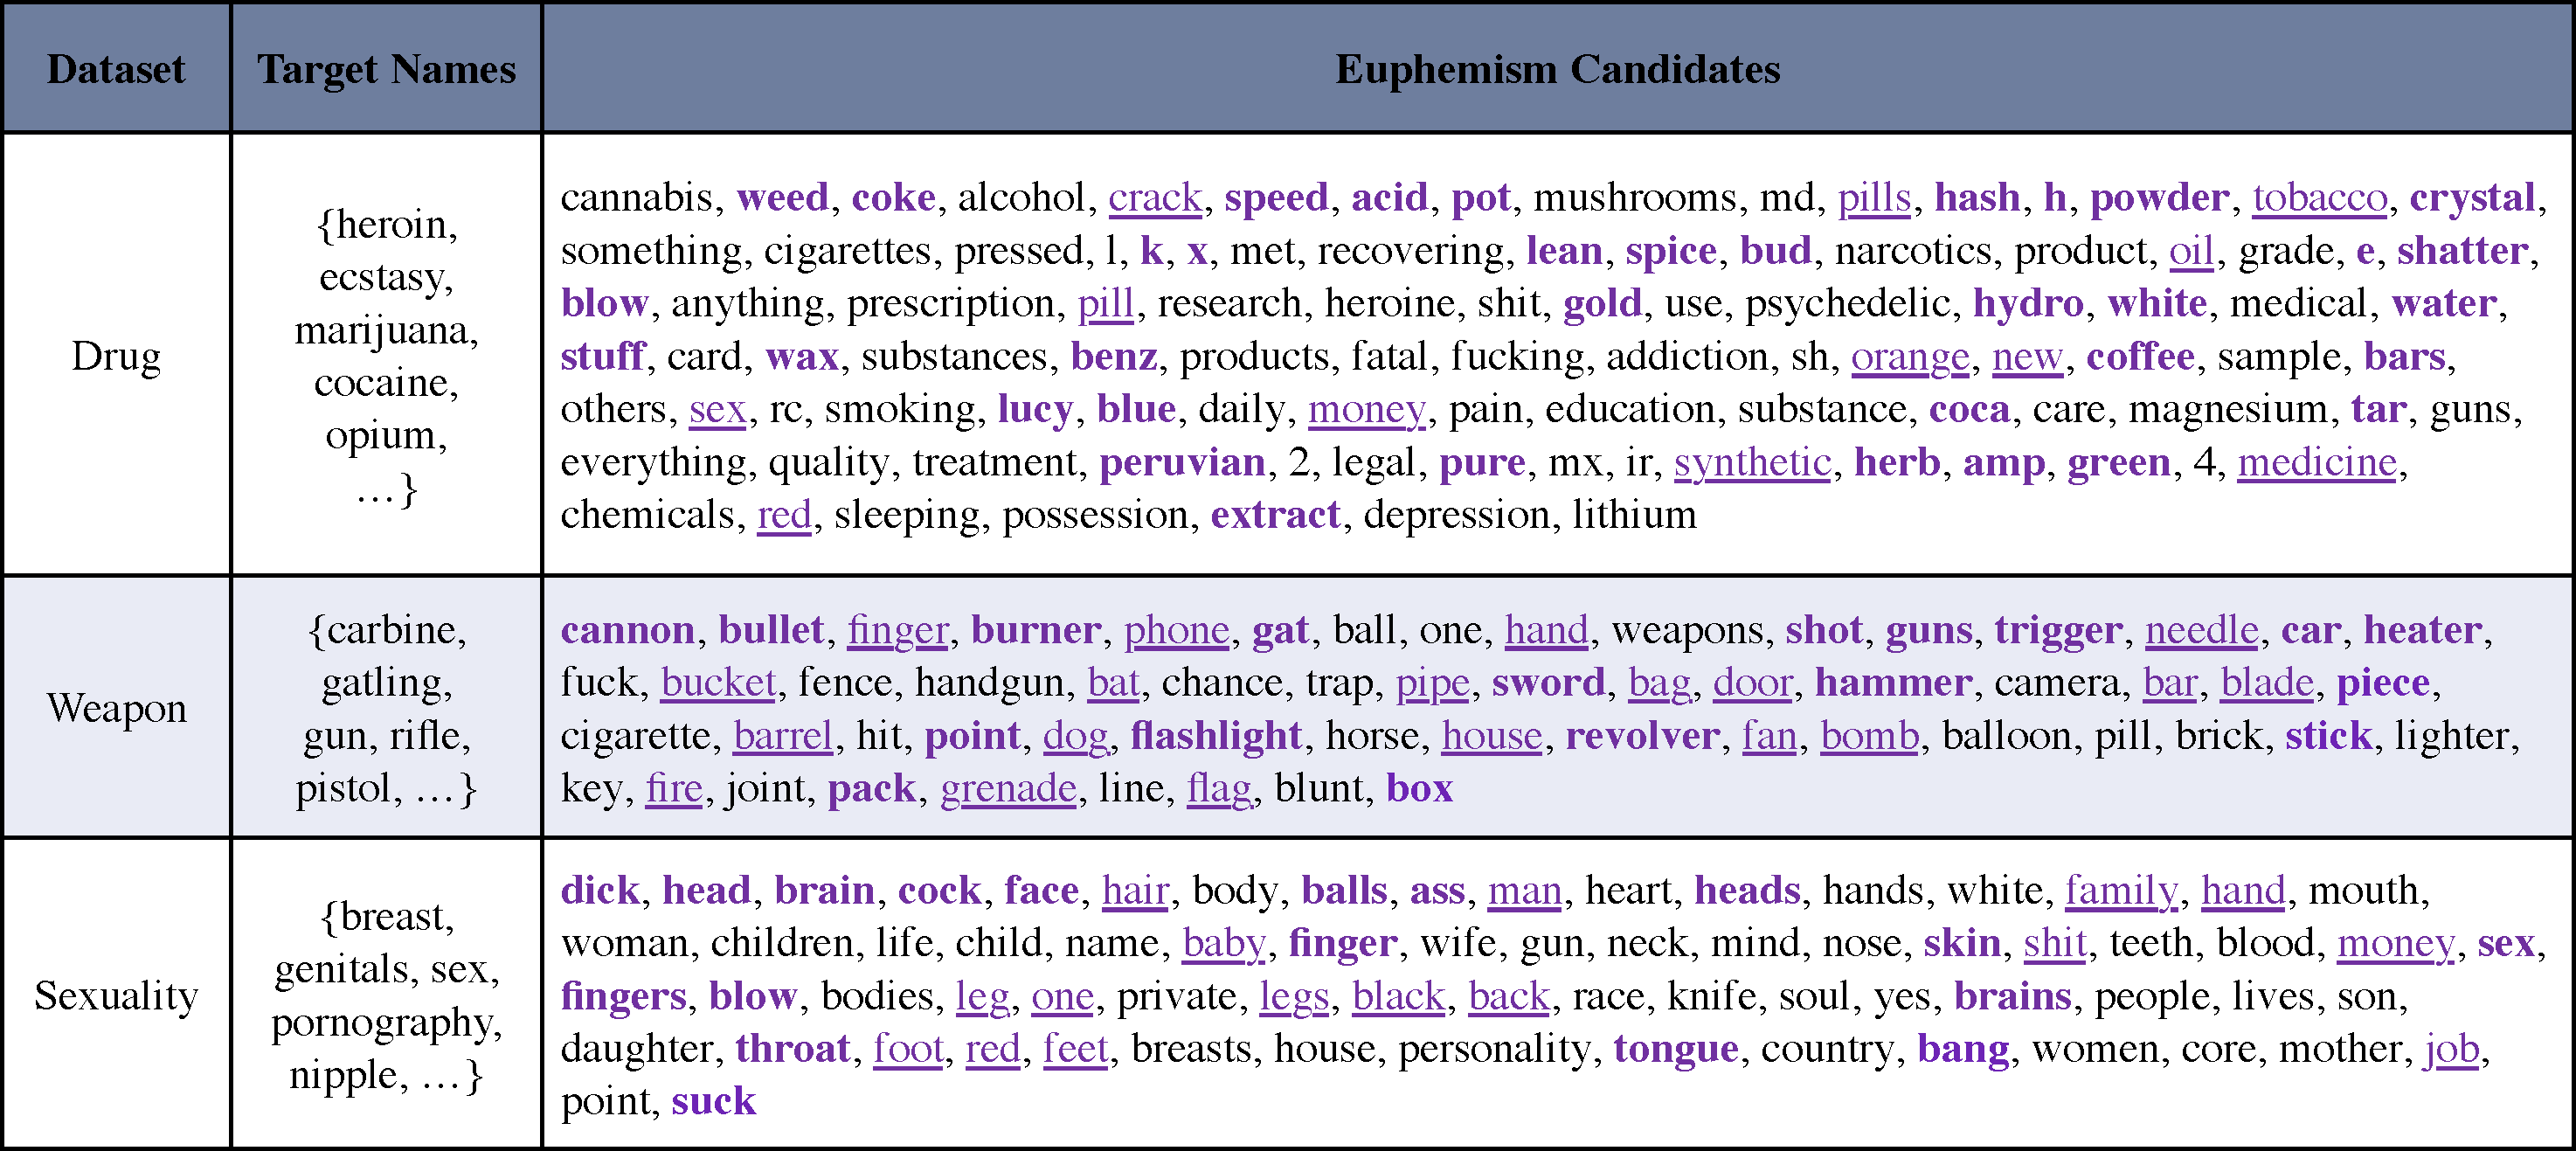
\includegraphics[width=1\linewidth]{figures/CaseStudies-Detection}
	\label{fig:casestudies-detection}
\end{table*}

\begin{table*}
	\centering
	\caption{Case studies of the false positive detection results on the drug dataset. They are real examples from Reddit.}
	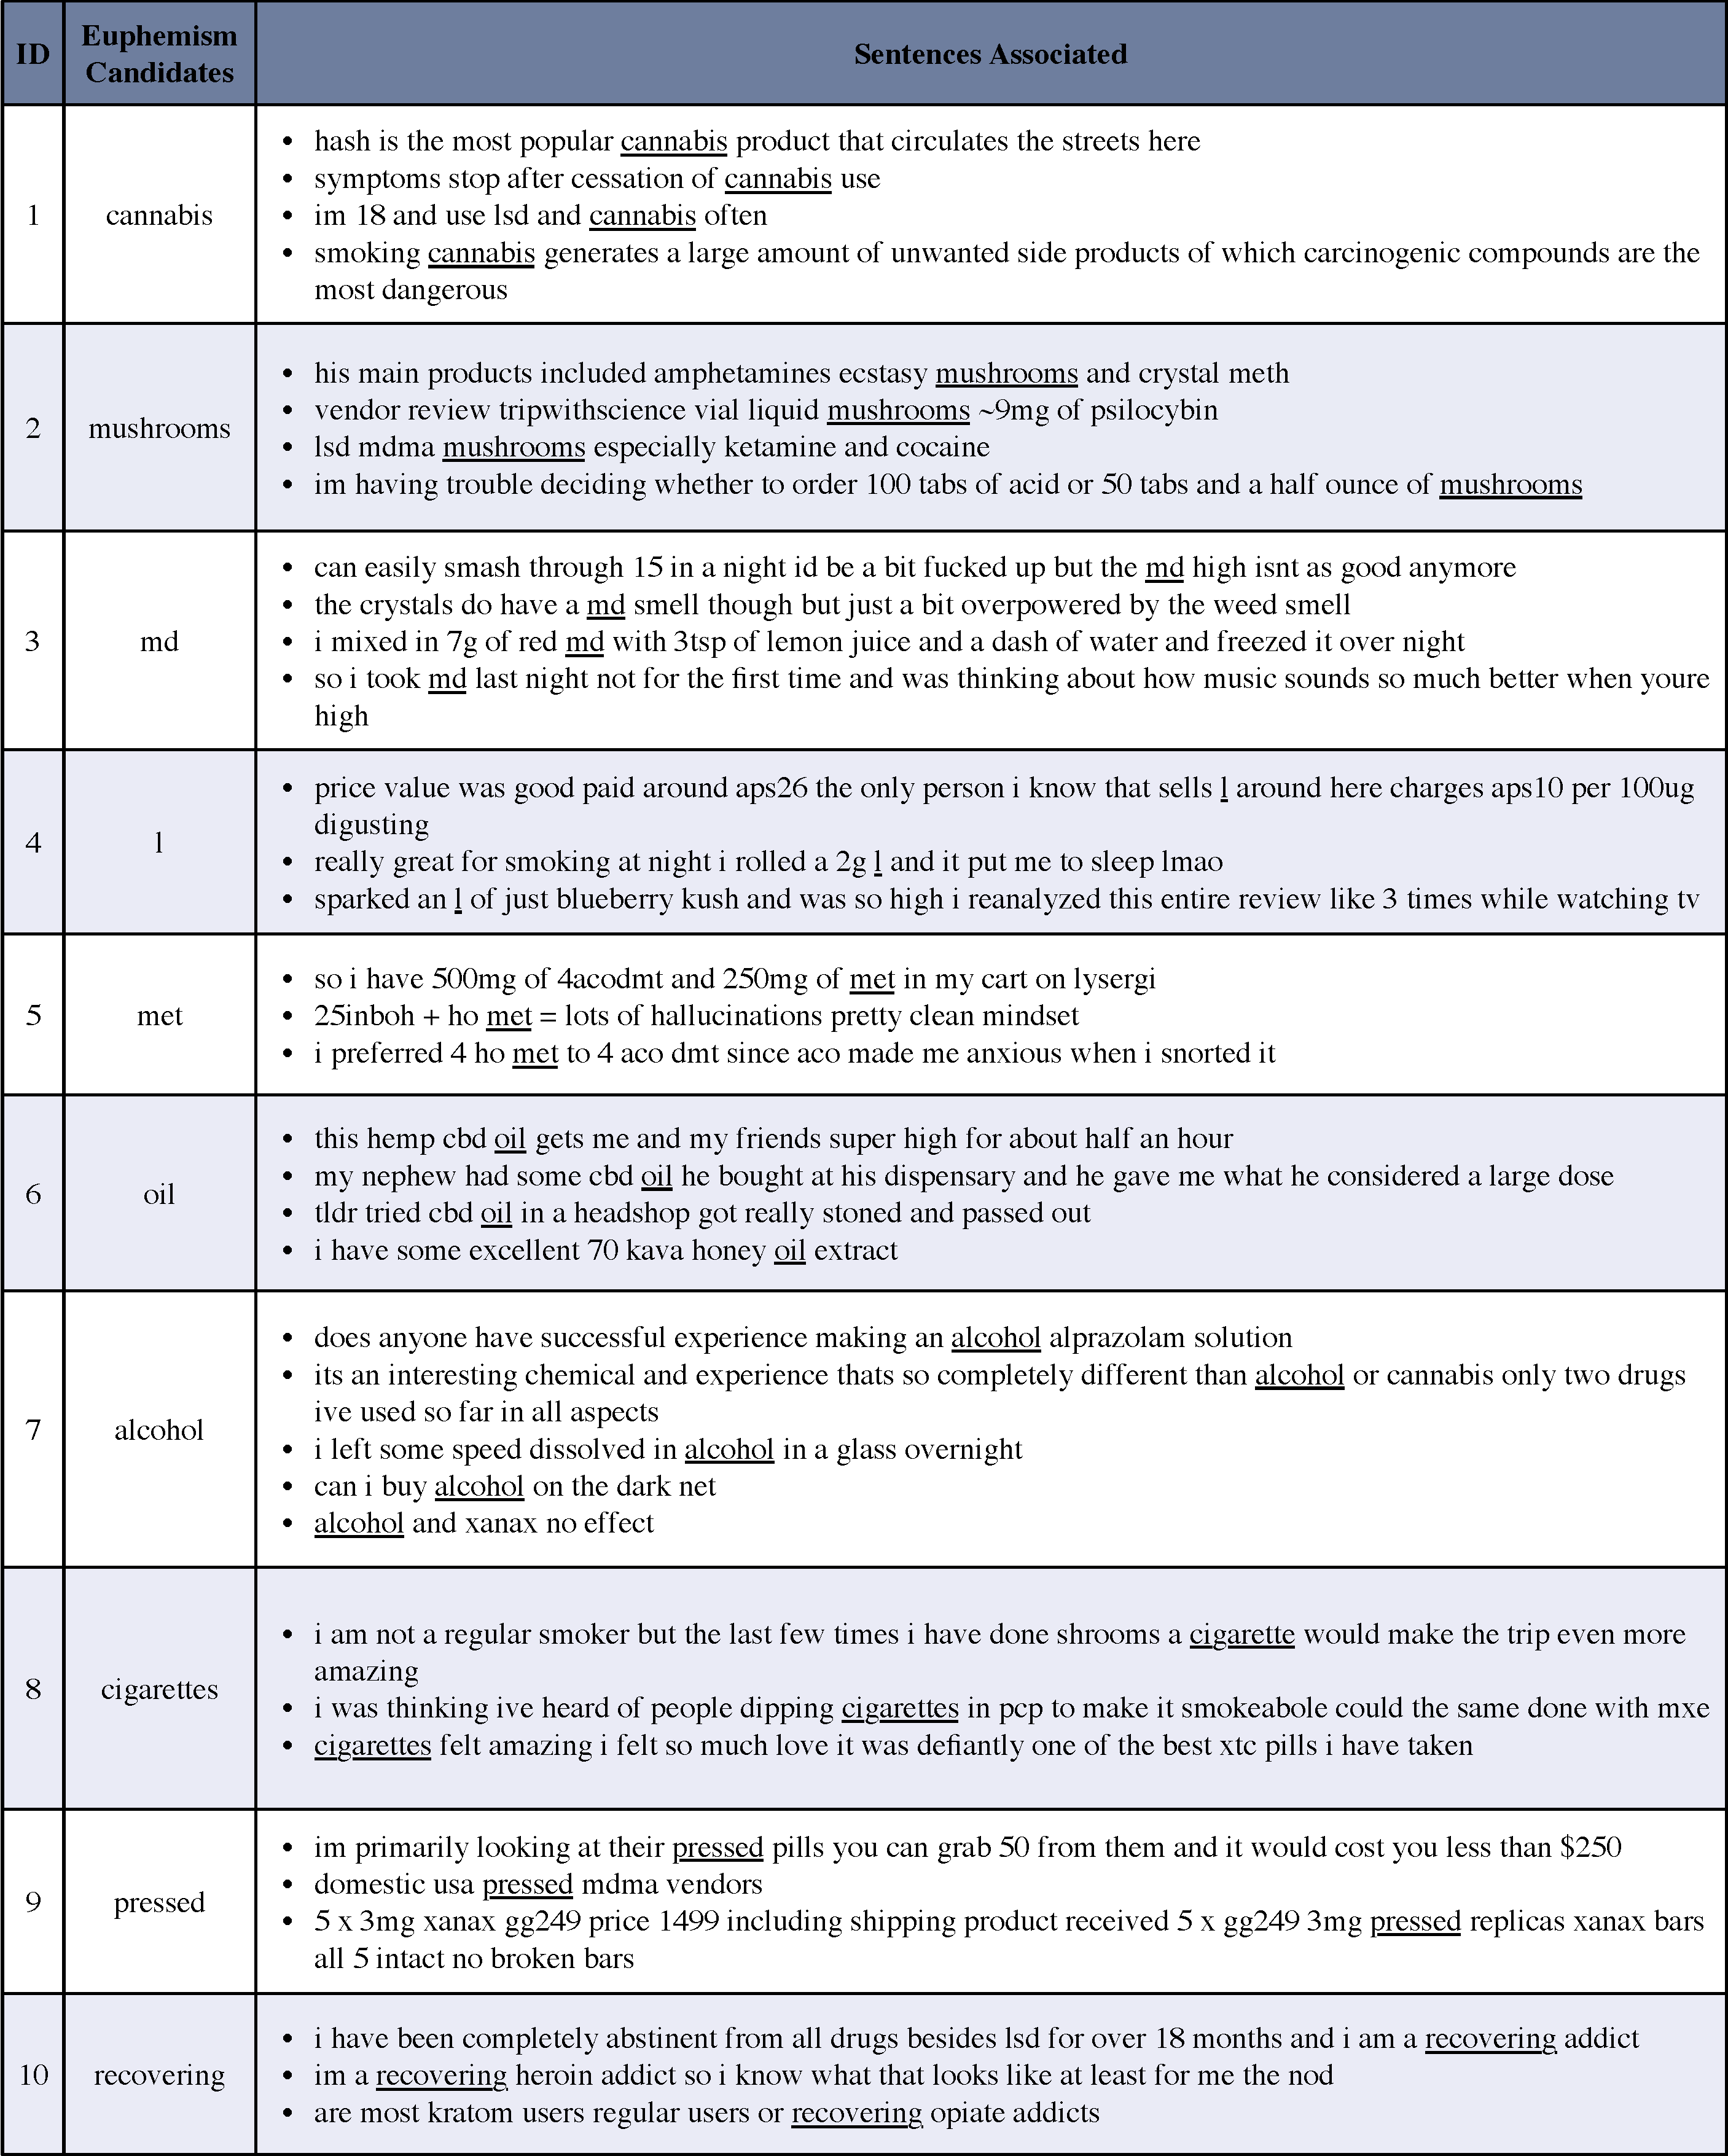
\includegraphics[width=0.96\linewidth]{figures/CaseStudies-Detection2}
	\label{fig:casestudies-detection2}
\end{table*}

\section{Case Study of Euphemism Detection}
\label{sec:appendix}

We present the euphemism detection results by our approach in Table \ref{fig:casestudies-detection} and analyze the false positive detection results on the drug dataset in Table \ref{fig:casestudies-detection2}. 
We categorize our false detection results into four types: 
\begin{itemize}
	\item They are correct euphemisms but missed on the ground truth list (cases 1-5 in Table \ref{fig:casestudies-detection2}). 
	\item They are not euphemisms by themselves, but they are contained in euphemism phrases. For example, as shown in case 6 in Table \ref{fig:casestudies-detection2}, ``oil'' is not a drug euphemism while ``cbd oil'' is one. 
	\item Though they are not euphemisms, they are strongly related to drug or the usage of drug (cases 7-10 in Table \ref{fig:casestudies-detection2}). Cases 7 and 8 uncovers some ways that people take drugs (together with alcohol or cigarettes).
	\item Incorrect detection. 
\end{itemize}

The case studies reveal that we can even find some correct euphemisms that are not on the ground truth list, which suggests the rapid-evolving nature of euphemisms and the necessity of the automatic euphemism detection task. 

	
\end{document}
